%                                   NADPIS                      
\chapter{Úvod}
\label{uvod}
Tato bakalářská práce se zabývá chytrými kartami Mifare Classic. Tyto karty jsou nejrozšířenější ve stále se zvyšujícím počtu bezkontaktních karet. Většina typů karet je navržena s požadavkem na co nejnižší cenu. To má za následek snížení zabezpečení těchto karet. Vyjímkou nejsou ani karty Mifare Classic. Navzdory tomu, že se jedná o jednu z nejrozšířenějších karet na světě, obsahuje velké množství zranitelností umožňující například kopírování obsahu karty. Tyto karty byly představeny v roce 1996. Netrvalo však dlouho a byly představeny první útoky, pomocí nichž je možné měnit obsah karty s pomocí jednoduchých čtecích zařizení. Hromadné využívání těchto útoků vedlo nákladným změnám bezpečnostních systémů mnoha firem.  Vzhledem k tomu, že karty Mifare Classic se hojně používají dodnes jako způsob identifikace osob, je toto téma stále zajímavé a aktuální. V této práci jsou vybrány tři různé zranitelnosti a jsou demonstrovány za pomoci nástroje Chameleon Mini. Kompaktní rozměry spolu s dostupností tohoto zařízení umožňují nejen penetrační testování přístupových systémů, ale také zneužitelnost osobami s nekalými úmysly.\par
Cílem práce je nejprve nastudovat technologi RFID, tedy technologii umožňující bezkontaktní komunikaci. Dále karty Mifare Classic se zaměřením na zabezpečení a zranitelnosti těchto karet. Praktickou částí je demonstrace vybraných zranitelností těchto karet. K demonstraci slouží zařízení Chameleon Mini, které bylo také nutné nastudovat. Po praktické části následuje analýza rizik využití provedených demonstrací v reálném prostředí.
\section*{Členění práce}
Druhá kapitola se zabývá principy technologie RFID, která je využívána jako komunikační rozhraní těchto karet. Je nastíněna stručná historie této technologie, využívané komponenty jako RFID čipy a čtecí zařízení a jiné využití v praxi.\par
V další kapitole je nejprve ujasněno, co to jsou chytré karty, následuje popis produktové značky Mifare a nakonec jsou podrobně popsány samotné karty Mifare Classic, jejich struktura paměti, šifrovací algoritmus a autentizační a komunikační protokol.\par
Čtvrtá kapitola popisuje vybrané zranitelnosti v návrhu karet Mifare Classic a jejich šifrovacím algoritmu CRYPTO1.\par
Pátá kapitola představuje zařízení Chameleon Mini, jeho schopnosti a podporované příkazy. 
V následující kapitole je dokumentováno testovací prostředí, ve kterém budou útoky provedeny. Kromě toho také nástroje vytvořené k usnadnění práce se zařízením Chameleon Mini.\par
Sedmá kapitola se zaobírá jednotlivými vybranými útoky. Je rozdělena na popis kryptografické analýzy, útok pomocí emulace karet a relay útok. Každá podkapitola obsahuje teoretický rozbor útoku a jeho průběh, nastavení zařízení Chameleon Mini a případnou implementaci útoku. Následuje samotné provedení útoku s popisem jeho průběhu a vyhodnocení. Vyhodnocení se také věnuje analýze provedení dané demonstrace v reálném prostředí.

%                                   NADPIS                      
\chapter{Radio frekvenční identifikace}
\label{technologie_rfid}
V této kapitole jsou popsány principy komunikace pomocí radio frekvenční identifikace (dále jen~RFID), její historie, jednotlivé komponenty a využití v průmyslu a každodenním životě.

\section{Úvod do RFID}
RFID je zkratka pro {Radio-Frequency IDentification}, tedy identifikace pomocí rádiové frekvence (dále jen~RF). Tato technologie umožňuje bezdrátovou komunikaci na relativně krátkou vzdálenost pomocí elektromagnetického pole. Jako RFID jsou popsány různé přístupy k identifikaci objektů, které pracují na různých frekvencích. Nejedná se tak o jedinou technologii, nýbrž o celý soubor identifikačních technologií. Různé alternativy jsou popsány mezinárodními standardy jako například ISO~14443, ISO~15693 nebo ISO18092. Technologie využívána k automatické identifikaci objektů, které jsou spojeny s RFID značkami, neboli tagy. Tyto tagy po přiblížení odpovídají RFID čtecímu zařízení. Vzdálenost na jakou mohou tag a čtecí zařízení komunikovat se liší na základě použité frekvence. Tagy ani čtecí zařízení většinou neobsahují žádnou logiku. Zprávu o načtení tagu předá čtecí zařízení {back-end} systému, který informaci zpracuje.\cite{The_RF_in_RFID}.\par
\par

\section{Historie}
Principy~RFID byly poprvé použity v systému~IFF (Identity: Friend or Foe) za 2. světové války Britskou armádou. Tento systém měl za úkol rozlišit vlastní letadla od nepřátelských. Proto byla vybavena nastavitelným {radio-majákem}, který byl schopen vysílat 6~identifikačních kódů. Systém pracoval v principu tak, že vysílač (radar) vyslal dotaz směrem k letadlu. Po dosažení a zpracování signálu odpovídač (transpondér) na letadle vyslal signál zpět, čímž došlo k zjištění příslušnosti stroje. Transpondér mohl odpovídat dvěma způsoby. Pasivní systém využil odražený původní signál a upravil ho tak aby obsahoval potřebné informace. Tento princip je dnes nejvíce využívaným způsobem identifikace pomocí RFID. Naopak aktivní systém přijal signál a sám okamžitě odeslal odpověď, přičemž ta mohla být odeslána i na jiné nosné frekvenci. V padesátých letech minulého století se radio identifikace rozmohla z armády do celého letectví a používá se dodnes. %\cite{The_RF_in_RFID}\cite{Emulator_UHD_RFID_Tagu}.
\par
RFID vznikla jako alternativa k čárovým kódům. I když je výroba čárových kódů levnější, mají proti RFID mnoho nevýhod. Pro čtení musí čtecí zařízení přímo vidět na štítek s kódem. Nesmí být snížená jeho vizuální čitelnost například špínou popisovačem nebo pokroucením. Zápis vícero informací se dá řešit pouze zvětšením plochy štítku nebo použitím jemnějšího značení, které je ale viditelné z menší vzdálenosti. Modifikace dat uložených pomocí čárových kódů se dá prakticky řešit pouze tiskem nového kódu \cite{The_RF_in_RFID}\cite{Emulator_UHD_RFID_Tagu}.

\section{Tagy}
Primární využití RFID tagů spočívá v identifikaci objektů. Cena takových objektů je nesrovnatelně vyšší oproti ceně tagu. Pokud je značený objekt levný, tag musí být ještě levnější. Na rozdíl od RFID~čteček jsou tagy prakticky pořád v pohybu, ať už jako chytré karty, nebo identifikátory zboží, vlaků kontejnerů apod. Tagy tedy musí být velmi levné za vysoké odolnosti proti fyzickému poškození\cite{The_RF_in_RFID}.
RFID~tag je systém skládající se minimálně z mikročipu, antény a pouzdra. Mikročip obsahuje pamět a logické obvody pro příjímání a odesílání dat čtecímu zařízení. Anténa přijímá signál z čtečky a poté jej zpětně rozptýlí (dále jen backscatter modulace) odesílanými daty. Pouzdro je potřeba pro udržení integrity tagu a jako ochrana proti vnějšímu poškození samotného čipu a antény\cite{RFID_explained}.
RFID tagy se dělí na aktivní, pasivní a částečně pasivní podle toho, zda je jsou napájeny z externího nebo interního zdroje\cite{The_RF_in_RFID}. Rozdíl je také v tom, kdo iniciuje komunikaci. Aktivní tag komunikaci zahajuje sám, zatímco komunikaci s pasivními tagy musí zahájit sama čtečka\cite{Hazardous_areas}. 

\subsection{Pasivní tagy}
\label{pasivniTagy}
Pasivní tagy identifikují levné objekty. Interní zdroj, i ve formě malé baterie, je pro ně příliš velký a drahý. Stejně jako transmittery a přijímače používané v klasických radiových zařízeních. Bez konvenčního zdroje energie jsou prakticky použitelné pouze jednoduché obvody, které je možno napájet bezdrátově i na vzdálenost několika metrů od čtecího zařízení. 
\par 
Aby mohl integrovaný obvod tagu pracovat, potřebuje zdroj stejnosměrného proudu několika desítek mikroampérů o napětí jeden až tři volty v závislosti na typu použitých tranzistorů. Toto napětí musí tag získat z RF signálu\cite{The_RF_in_RFID}. Frekvence tohoto signálu se podle použití liší. Od použité frekvence se také odvíjí dosah čtení a rychlost přenosu dat. Používané frekvence spadají do několika pásem, a to nízká frekvence ({Low Frequency - LF}), vysoká frekvence ({High Frequency - HF}) a ultra vysoká frekvence ({Ultra High Frequency - UHF}). Evropská a americká specifikace pásma~UHF se liší ve frekvenci (viz. tabulka \ref{tabulka_pasem}). Chytré karty používají HF~pásmo\cite{Smart_Cards_Tokens_Security}. \par
\begin{table}[]
\begin{tabular}{cccc}
\hline
Pásmo               & Frekvence   & Dosah   & Přenosová rychlost \\ \hline
LF                  & 125-135 kHz & 1-2 m   & 100 bps            \\
HF                  & 13,56 MHz   & 2 m     & 2 kbps             \\
UHF-Evropa          & 865-868 MHz & 12-20 m & 40-640 kbps        \\
UHF-Severní Amerika & 902-928 MHz & 12-20 m & 40-640 kbps        \\ \hline
\end{tabular}
\caption{Porovnání vlastností operačních pásem RFID\cite{RFID_explained}\cite{The_RF_in_RFID}}
\label{tabulka_pasem}
\end{table}

Energie se přenáší na principu takzvaných volně vázaných transformátorů. Cívka ve čtecím zařízení generuje vysokofrekvenční elektromagnetické pole s vlnovou délkou 22m až 2400m. Vlnová délka nosné vlny je tedy mnohem delší než vzdálenost karty. To umožňuje volné vázání. Magnetické pole cívky v okolí čtecího zařízení indukuje napětí v cívce karty. Toto napětí je použito k napájení cívky. Účinnost tohoto modelu je velmi malá.\cite{Smart_card_handbook}\par
K přenosu dat čtecího zařízení kartě se využívá klíčování s amplitudovým, frekvenčním i fázovým posuvem. Tedy reprezentace digitálních dat pomocí příslušné modulace nosné vlny. K přenosu dat opačným směrem od karty ke čtecímu zařízení se využívá amplitudová modulace. Karta v poli čtecího zařízení využívá jeho energie. Změnou zatížení cívky v kartě lze měnit napětí na cívce čtecího zařízení. Tyto změny lze detekovat a interpretovat jako data. Změna zátěže v kartě je generována připojováním nebo odpojováním rezistoru z obvodu karty na základě datového signálu.\cite{Smart_card_handbook}\par

\begin{figure*}[ht]\centering
  \centering
  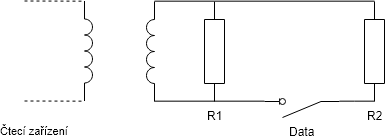
\includegraphics[width=0.7\linewidth]{obrazky-figures/obrazekRFIDDataTransfer.png}\\[1pt]  
  \caption{Princip přenosu dat karty}    
  \label{obrazekRfidPrincipPřenosuDat}
\end{figure*}

\subsection{Aktivní tagy} 
Aktivní tagy jsou napájeny z vlastního zdroje. Ten může být buď baterie, nebo připojení do elektrické infrastruktury. Zdroj napájí nejenom přenos dat, ale i ostatní elektronické komponenty. Těmito komponenty mohou být různé senzory nebo uživatelské rozhraní\cite{RFID_explained}. Vzhledem k technologii logických obvodů postupuje vývoj baterií velmi pomalu. Jedním z hlavních problémů návrhu těchto tagů je tedy zkrácení doby aktivity a snížení energie potřebné jak pro aktivní, tak pro klidové období tagu. Technologické skloubení těchto požadavků není jednoduché a výroba tagů se do jisté míry podobá výrobě běžných rádiových zařízení. Diskrétní komponenty a integrované obvody připájené k tištěným spojům, to celé připojené k anténě a uložené v plastovém krytu\cite{The_RF_in_RFID}. 
Částečně pasivní tagy obsahují vnitřní zdroj pouze k napájení pomocných komponent. Data jsou přenášena pomocí backscatter modulace jako u pasivních tagů\cite{Survey_of_RFID_Tags}.


\section{Čtecí zařízení}
Pro rádiovou komunikaci s tagy se používá čtecí zařízení, které funguje jako vysílač i přijímač dohromady. Taková zařízení komunikují buď plným, nebo polovičním duplexem. Poloduplexní spojení znamená, že zařízení nemůže přijímat a vysílat zároveň. Současný obousměrný přenos podporuje plný duplex. Pro komunikaci s pasivními tagy se používá právě plný duplex. Čtecí zařízení musí vysílat RF~signál pro napájení tagu a zároveň přijímat odpověď.
Nedílnou součástí čtecího zařízení je anténa. Vysílač i přijímač mohou mít každý svou anténu. Tato konfigurace je známá jako bistatická. Monostatický systém používá jednu anténu pro vysílání a přijímání signálu zároveň. V tomto případě je příjímač vystaven signálu z vysílače. Přijímač tedy musí být navržený tak, aby rozeznal signál z tagu\cite{The_RF_in_RFID}.\par

\section{Použití}
Technologie RFID nabízí mnohá využití v různých oblastech lidské činnost. Nejčastější je prevence chyb. Například ve zdravotnictví každý pacient dostane náramek obsahující RFID čip s pamětí. Do paměti jsou pak ukládány informace o pacientovi, jeho patologie, předepsané a podáné léky a jiné skutečnosti. Jedním z nejznámějších využití je sledování zboží a ochrana proti jeho krádeži. Zboží je opatřeno identifikátorem, který obsahuje data o přijetí do skladu či obchodu. Vstupy a výstupy budovy jsou opatřeny čtecími zařizeními, které registrují procházející zboží. Stejné značky lze využít v pokladnách při prodeji zboží. Značka obsahuje cenu, kterou odečte čtecí zařízení pokladny a přičte ji na účet zákazníka. Zároveň může být na zboži deaktivována ochrana, která by způsobila poplach při průchodu branou vybavenou čtečkou bez zaplacení.\cite{BezpecnostRfid}\par

%                                   NADPIS                      
\chapter{Chytré karty Mifare Classic\textsuperscript{\textregistered}}
\label{chytre_karty}
V této kapitole jsou popsány obecně chytré karty a jejich typy. Následuje popis komunikačních standardů chytrých karet a představení značky Mifare. Následuje podrobný popis karet Mifare Classic, jejich struktura paměti, využitý algoritmus CRYPTO1, autentizační fáze karty a její komunikační protokol.

\section{Co jsou chytré karty}
Chytré karty, jak už název napovídá, jsou karty, které mohou být použity chytrým způsobem. Za chytrou kartu považujeme plastovou kartu s integrovaným obvodem. Takové karty lze obecně považovat za čipové karty a ty mohou být v kontaktní nebo bezkontaktní variantě. Kontaktní karty se vkládají do čtecích zařízení, které naváže fyzický kontakt se zlatě zbarveným rozhraním karty. Bezkontaktní karty stačí dostat do blízkosti čtecího zařízení. Napájení a komunikace je poté zajištěna pomocí~RFID. Pod pojmem ''chytrá karta'' si obyčejně člověk představí platební kartu. Chytré karty mohou ale být použity i ve formě elektronických pasů, občanských průkazů, přístupových karet, jsouvhodné jako zabezpečení proti krádeži apod. Ne~každá karta vyžaduje stejné zabezpečení. Některé ho nevyžadují vůbec, například jednoduché tagy vysílající své~ID jako inventarizační systém ve skladech. Jiné vyžadují složité kryptografické mechanismy zajišťující soukromí přenášených dat. 
\par
Jednoduchý tag je z těchto produktů nejméně zabezpečený. Je nastaven tak, že své unikátní identifikační číslo (dále jen~UID), které vysílá, je pouze pro čtení {(Read-only)}. Kromě vysílání svého~UID nemá žádný jiný protokol, je tedy jednoduché odposlouchávat komunikaci a replikovat ji pomocí emulátoru. Místo speciálního emulátoru lze použít podobný tag, který umožnuje změnu svého UID.
\par
Paměťové tagy, stejně jako jednoduché, mají~UID, navíc ale obsahují paměť. Tato paměť je jak pro čtení, tak pro zápis {(Read/Write)}. Její přenos není nijak šifrován, což může vést k neoprávněnému čtení nebo emulaci. Výrobce karet může ovšem data opatřit ochranou integrity, například pomocí MAC (z anglického Message Authentication Code). Tato metoda zabrání útočníkovi ve vytváření nových a modifikaci stávajících dat. Je ale nutné opatřit čtecí zařízení funkcionalitou a klíči k ověření MAC\cite{Mifare_Classic_story}.
\par
MAC je krátká informace odesílána s daty, která dokáže zajistit integritu a autenticitu dat. To znamená ověřit, že data byla odeslána důvěryhodným odesílatelem a nebyla nijak modifikována. Jedná se o metodu výpočtu kontrolního součtu s pomocí symetrické kryptografie. Tato metoda se skládá ze tří algoritmů. První algoritmus generuje náhodné klíče z množiny klíčů. Druhý algoritmus na základě vstupních dat a sdíleného tajného klíče vygeneruje~MAC. A třetí algoritmus pomocí klíče a MAC verifikuje přijatá data\cite{Foundations_Of_Cryptography}.
\par
Tag se zabezpečenou pamětí implementuje nějaký kryptografický protokol pro správu přístupu k paměti. Tag a čtecí zařízení se nejprve vzájemně autentizují a teprve poté je povolen přístup k paměti. Data z paměti jsou před odesláním většinou nejprve zašifrována relačním klíčem, aby byla zajištěna jejich bezpečnost. Paměť některých tagů je rozdělena do menších oddílů, z nichž každý má vlastní klíč. Toto uspořádání umožňuje použít jeden tag k více aplikacím, přičemž každé aplikaci náleží jiný klíč.
\par
Nejpokročilejšími jsou zabezpečené tagy s mikrokontrolerem, který umožňuje nahrát různou funkcionalitu. Tyto tagy obvykle implementují bezpečnostní standardy jako například Global Platform. Šifrování, verifikace a další symetrické i asymetrické kryptografické metody jsou zajištěny kryptografickými koprocesory přímo na tagu\cite{Mifare_Classic_story}. Správný chod mikrokontroleru je zabezpečen například senzory vysokého a nízkého napětí, teploty nebo frekvence, filtrem vstupu hodinového signálu nebo aktivním stíněním\cite{NXP_Microcontroller_overview}.

\section{Standardy komunikace chytrých karet}
Standard ISO~14443 je určena zejména pro identifikační a platební karty. Skládá se ze čtyř částí. První část s označením {ISO~14443-1} popisuje zejména fyzikální charakteristiky karty, její velikost a odolnost proti mechanickému namáhání a působení elektrických a magnetických polí. Druhá část ({ISO~14443-2}) udává charakteristiky elektromagnetického pole, které zajišťuje napájení a obousměrnou komunikaci mezi čtecím zařízením a kartou. Čtecí zařízení je zde označováno jako~PCD, tedy Proximity Coupling Device, a karta jako~PICC, což je zkratka pro Proximity Integrated Circuit Card. Zde jsou také definovány dvě metody přenosu dat, typ A a typ B. Ty se liší v kódování a v modulaci frekvencí. Třetí část ({ISO~14443-3}) uvádí, jak má čtecí zařízení postupovat při inicializaci komunikace s kartou, tedy formát bytů, časování a obsah příkazů REQ a ATQ. Dále popisuje, jak detekovat a komunikovat pouze s jednou kartou z mnoha v dosahu zařízení, antikolizní metody. Poslední část ({ISO~14443-4}) popisuje protokoly a příkazy používané na vyšších vrstvách komunikace po inicializaci\cite{ISO14443}.
\par
Některé zprávy obsahují takzvaný cyklický redundantní součet (dále jen~CRC, z anglického Cyclic redundancy check). Je to metoda používaná k detekci chyb, nemůže být ovšem použita k jejich korekci. Součet generuje cyklický posuvný registr se zpětnou vazbou. Parametry registru (a~výpočtu) se mění v závislosti na typu této metody. Standard ISO 14443 používá CRC typu~A. Registr má 16~bitů s počáteční hodnotou~$0x6363$ a generačním polynomem $C(x) = x^{16} + x^{12} + x^5 + 1$. Výsledek metody se přidá na konec zprávy. Po přijetí zprávy je kontrolní součet znovu, nezávisle spočítán stejnou metodou. Pokud se vypočítaný součet liší od přijatého, nastala při přenosu chyba\cite{Smart_card_handbook}\cite{ISO14443}.


\section{Mifare\textsuperscript{\textregistered}}
Mifare\textsuperscript{\textregistered} je obchodní značka rakouské společnosti NXP Semiconductors, dříve známé pod jménem Philips Semiconductors. Tato značka zahrnuje množství proprietárních, bezdrátových řešení splňující mezinárodní standard~ISO/IEC~14443. Produktová rodina zahrnuje čtyři typy karet. Zpětná kompatibilita zajišťuje bezproblémové přecházení na lépe zabezpečené produkty s více funkcemi. S více než 10~miliardami prodaných karet ovládá Mifare zhruba 80\% světového trhu s bezdrátovými chytrými kartami. 
\cite{About_Mifare}\cite{Dismantling_Mifare_Classic}.

\subsection{Varianty karet Mifare}

Karty Mifare Classic\textsuperscript{\textregistered} byly vyvinuty již v roce~1994 a brzy se staly úspěšným produktem. Původně byly navrženy jako karty se zabezpečenou pamětí. Byly proto používány v různých odvětvích, například v hromadné dopravě, ve školních kampusech nebo jako zaměstnanecké karty. Data a autentizace jsou šifrovány proprietární šifrou CRYPTO1. Zabezpečení ale není nejsilnější stránkou těchto karet. Pro porovnání i mnohem starší DES~šifrování odolá o několik řádů déle útokům hrubou silou (brute force). Toho si je firma vědoma a nadále tyto karty nedoporučuje pro aplikace s důrazem na zabezpečení. Požadavky na bezpečnost vedly k vývoji dvou nových, lépe zabezpečených typů karet Mifare Plus a Mifare DESFire\cite{Mifare_Classic_story}\cite{Mifare_Classic_Official_about}. 
\par
Chytré karty Mifare Plus\textsuperscript{\textregistered} jsou nástupcem karet Classic. Zpětná kompatibilita je zajištěna podporou starší a méně bezpečné šifry CRYPTO1. Je tedy možné postupně modernizovat již zavedené systémy, i když tento způsob neodstraňuje všechna rizika karet Classic. Navíc je implementována mnohem bezpečnější 128bitová AES~šifra. Karty Mifare DESFire\textsuperscript{\textregistered} už šifrování CRYPTO1 nepodporují vůbec. Podporují ovšem šifrování~DES~a~AES, komunikaci pomocí~NFC a až 28~různých aplikací na jedné kartě\cite{Mifare_Classic_Official_about}. V~České Republice je používají například České dráhy ve svém produktu In Karta\cite{Ceske_Drahy_Podminky_InKarta}. Naopak Ultralight\textsuperscript{\textregistered} jsou velmi levné karty s krátkou životností a malou pamětí. Jsou vhodné pro jednorázové použití jako celodenní jízdenky nebo vstupenky na velké události\cite{Mifare_Classic_Official_about}. Každá z těchto karet se dělí na další dva až čtyři podtypy, které se liší v různých parametrech nebo nabízených vlastnostech karty.

\begin{table}[]
\begin{tabular}{lllll}
\hline
Produkt     & Rychlost přenosu  & Velikost paměti   & Šifrování                 & Životnost \\ \hline
Classic\textsuperscript{\textregistered}     & 106 kbps          & 1-4 KB            & CRYPTO1                   & 10 let    \\
Plus\textsuperscript{\textregistered}       & 106-848 kbps      & 2-4 KB            & CRYPTO1, 128 bit AES      & 10 let    \\
DESFire\textsuperscript{\textregistered}     & 106-848 kbps      & 256 B - 8 KB      & 128 bit AES, 168 bit DES  & 10 let    \\
UltraLight\textsuperscript{\textregistered}  & 106 kbps          & 40-144 B          & 112 bit DES               & 2 roky    \\ \hline
\end{tabular}
\caption{Porovnání jednotlivých Mifare karet\cite{Vedeckotechnicky_sbornik_cd}}
\label{tabulka_Mifare_karet}
\end{table}

\section{Karty Mifare Classic}
Jak již bylo řečeno, Classic jsou karty se zabezpečenou pamětí. Data udržuje čip s pamětí typu EEPROM. To je zkratka pro Electrically Erasable Programmable {Read-Only} Memory, tedy elektronicky mazatelná a programovatelná paměť pouze pro čtení. Důležitou vlastností je, že EEPROM je nevolatilní paměť, svůj stav si udrží i bez zdroje napájení\cite{Smart_card_handbook}. Nad pamětí karty Classic lze provádět základní operace jako čtení, zápis, přičtení a odečtení. Paměť karty je rozdělena do sektorů a sektory jsou dále rozděleny do bloků po 16 bytech. Na prvním bloku prvního sektoru je zapsáno UID~karty, kontrolní součet a data výrobce. Poslední blok každého sektoru obsahuje dva 48bitové klíče a podmínky přístupu pro daný sektor. Klíče jsou sdíleny s legitimním čtecím zařízením. To se musí autentizovat alespoň jedním z nich. Podmínky přístupu říkají, se kterým klíčem lze provádět jaké operace\cite{Dismantling_Mifare_Classic}\cite{Mifare_Classic_story}.
\par

\subsection{Struktura paměti} % (fold)
\label{sub:struktura_paměti}
Paměť karet je rozdělena do sektorů a ty jsou dále děleny do bloků po 16~bytech. Karta Mifare Classic~1k disponuje 16~sektory, a každý z nich má 4~datové bloky. Struktura karet Mifare Classic~4k je více heterogenní. Prvních 32 sektorů se skládá ze 4~datových bloků a zbývajících 8~sektorů obsahuje bloků~16. První blok prvního sektoru obsahuje speciální data. Na prvních 4~bytech je zapsán unikátní identifikátor (UID)~karty. Následuje jednobytová bitová kontrola počtu (dále jen~BCC z anglického bit count check). Ta se vypočítá postupným provedením operace~XOR nad všemi byty~UID. Na zbývajících bytech jsou uložena data výrobce. Celý tento blok je pouze pro čtení. 

\begin{figure*}[ht]\centering
  \centering
  \hspace*{-0.07\linewidth}
  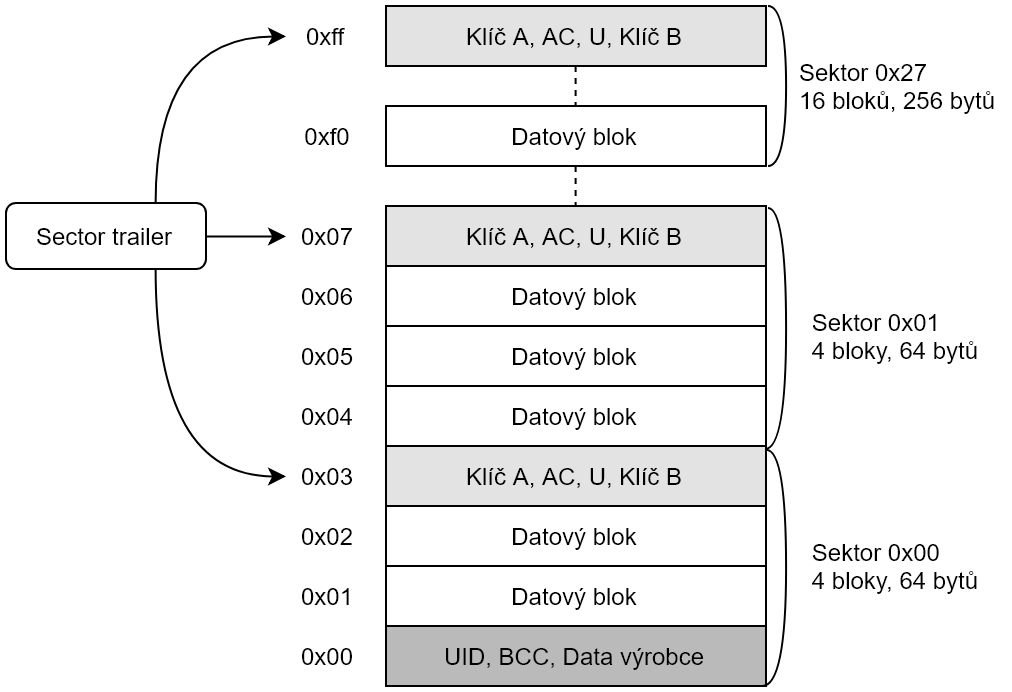
\includegraphics[width=0.6\linewidth,height=180px]{obrazky-figures/MemoryStructure.png}\\[1pt]  
  \caption{Struktura paměti karty Classic\cite{PracticalAttackOnMifare}}    
  \label{obrazekStrukturaPametiKarty}
\end{figure*}

\par
Před jakoukoliv operací nad pamětí karty se čtecí zařízení musí nejprve autentizovat proti sektoru, se kterým chce pracovat. Každý sektor uzavírá takzvaný sector trailer, speciální datový blok. Obsahuje tajné klíče~A~a~B, které jsou použity při autentizaci. Operace, které je možné nad sektorem provádět, jsou v podmínkách přístupu~AC (z anglického Access Condition). Poslední částí sector traileru je jeden datový byte~U, který nemá definovaný účel. Může však být použit pro uložení dat. Sector trailer má zvláštní podmínky přístupu. Zatímco klíč~A není čitelný nikdy, klíči~B se čitelnost nastavit může. V takovém případě se jím nedá autentizovat a je považován za uživatelská data. Čitelností klíče je myšlen přístup čtecího zařízení k tomuto datovému prostoru s právy pro čtení, karta samotná je může číst bez problémů\cite{PracticalAttackOnMifare}. \par
Nastavení klíčů a podmínek přístupu se provede jednoduchým zápisem dat do sector traileru. Nejmenší jednotka přístupu je však celý blok. Načítání nebo zápis tedy přečte, respektive přepíše blok celý. Změna jediného bytu vyžaduje načtení a~přepsání celého bloku. Pro sector trailer je tato operace o~něco složitější. Čtení bytů na pozicích, kde jsou uloženy klíče, vrací nuly. Tedy změna konfigurace beze změny klíčů vyžaduje znalost těchto klíčů. Takže například nelze zjistit neznámý klíč B změnou konfigurace podmínek přístupu~AC a jeho následným přečtením, protože změna AC vyžaduje přepsání celého bloku i s klíčem\cite{makingTheBestOf}.
\par
Na datových blocích jsou uložena libovolná data, nebo jsou konfigurovány jako blok s hodnotou (value block). Při použití hodnotového bloku je 4bytová podepsaná hodnota uložena dohromady třikrát. Dvakrát normálně a jednou invertovaně, tedy se všemi bity negovanými. Tyto 4~byty mají uložen nejvýznamnější byte vpravo a nejméně významný vlevo ({little-endian}). Na posledních čtyřech bytech je uložena jednobytová adresa bloku, která může být použita jako ukazatel. Adresa je uložena čtyřikrát po sobě, z toho druhý a čtvrtý byte jsou opět negovány\cite{PracticalAttackOnMifare}.

\begin{figure*}[ht]\centering
  \centering
  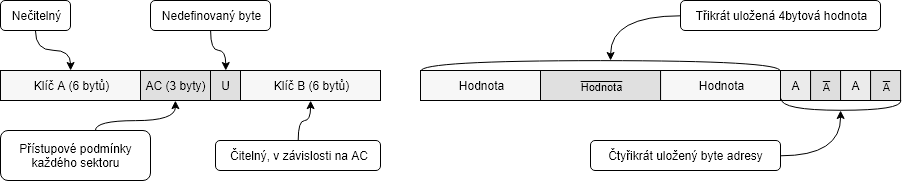
\includegraphics[width=\linewidth]{obrazky-figures/LogicalStructureBetter.png}\\[1pt]  
  \caption{Struktura paměti sector traileru a bloku s hodnotou\cite{PracticalAttackOnMifare}}    
  \label{obrazekStrukturaSpecialnichBloku}
\end{figure*}

\subsection{CRYPTO1}
\label{crypto1section}
Po autentizaci je veškerá komunikace mezi čtecím zařízením a kartou šifrována. Pro šifrování se používá proprietární proudová šifra CRYPTO1 navržena přímo firmou~NXP\cite{Mifare_Classic_story}. Proudové šifry jsou symetrické šifry kde je důvěrný text neznámé délky (anglicky plaintext) bit po bitu kombinován s proudem pseudonáhodných šifrovacích bitů (dále jen anglicky keystream). Kombinace se nejčastěji provádí pomocí funkce~XOR a jejím výsledkem je zašifrovaný text (cipher text). Šifrovaný text je dešifrován stejnou funkcí a keystreamem. Keystream i důvěrný text musí být stejně dlouhé. Aby bylo možné tohoto dosáhnout s konečnou pamětí, je potřeba keystream generovat. To se děje na základě klíče (anglicky secret key) v generátoru\cite{Stream_ciphers}. Šifra CRYPTO1 jako generátor používá 48bitový posuvný registr s lineární zpětnou vazbou (dále jen LFSR, z anglického Linear Feedback Shift-register) s generačním polynomem~\ref{generatingPolynomial}. Každou periodu hodinového signálu se z dvaceti určitých bitů pomocí filtrační funkce~\ref{filterFunction} vypočítá bit keystreamu a potom se všechny bity registru posunou doleva. Bit nejvíce vlevo je zahozen a nový, pravý bit je jako zpětná vazba vypočítán funkcí~\ref{feedbackFunction}, kde $x$ je aktuální stav registru. V průběhu inicializace se bere v úvahu také vstupní bit, který je kombinován funkcí XOR s~\ref{feedbackFunction}. \cite{Dismantling_Mifare_Classic}.

\begin{multline}
    \label{generatingPolynomial}
    g(x) = x^{48} + x^{43} + x^{39} + x^{38} + x^{36} + x^{34} + x^{33} + x^{31} + x^{29} + x^{24} + \\
     x^{23} + x^{21} + x^{19} + x^{13} + x^{9} + x^{7} + x^{6} + x^{5} + 1  % generating polynomial z dismantling
\end{multline}
\begin{multline}
    \label{feedbackFunction}
    L(x_0, x_1 \dots x_{47}) = x_{0} \oplus x_{5} \oplus x_{9} \oplus x_{10} \oplus x_{12} \oplus x_{14} \oplus x_{15} \oplus x_{17} \oplus x_{19} \oplus x_{24} \oplus \\ 
    x_{25} \oplus x_{27} \oplus x_{29} \oplus x_{35} \oplus x_{39} \oplus x_{41} \oplus x_{42} \oplus x_{43}
\end{multline}
\begin{multline}
    \label{filterFunction}
    f(x_0, x_1 \dots x_{47}) = f_c(f_a(x_{9},x_{11},x_{13},x_{15}),
                               f_b(x_{17},x_{19},x_{21},x_{23}),
                               f_b(x_{25},x_{27},x_{29},x_{31}), \\
                               f_a(x_{33},x_{35},x_{37},x_{39}),
                               f_b(x_{41},x_{43},x_{45},x_{47}))
\end{multline}
\begin{multline}
    \label{filterFunctionC}
    f_c(y_0,y_1,y_2,y_3,y_4) = 
    (y_0 \lor ((y_1 \lor y_4) \land (y_3 \oplus y_4))) \oplus \\
    ((y_0 \oplus(y_1 \land y_3)) \land ((y_2 \oplus y_3) \lor (y_1\land y_4)))
\end{multline}
\begin{equation}
    \label{filterFunctionA}
    f_a(y_0,y_1,y_2,y_3) = 
    ((y_0 \lor y_1) \oplus (y_0 \land y_3)) \oplus (y_2 \land ((y_0 \oplus y_1) \lor y_3))
\end{equation}
\begin{equation}
    \label{filterFunctionB}
    f_b(y_0,y_1,y_2,y_3) = ((y_0 \land y_1) \lor y_2) \oplus ((y_0 \oplus y_1) \land (y_2 \lor y_3))
\end{equation}

\begin{figure*}[ht]\centering
  \centering
  
  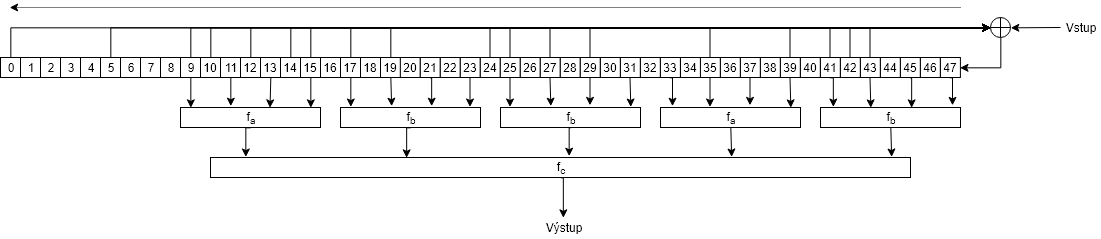
\includegraphics[width=\linewidth]{obrazky-figures/StrukturaSifry.png}\\[1pt]  
  \caption{Struktura šifry CRYPTO1\cite{Wirelessly_Pickpocketing}}    
  \label{obrazekStrukturaSifry}
\end{figure*}

\par
Inicializace šifry probíhá při autentizaci karty a čtecího zařízení. Poté, co karta odešle výzvu $n_T$ (viz kapitola \ref{autentizace}) je do registru šifry obou zařízení načten sdílený tajný klíč $K$. Zde přichází na řadu vstupní bit, který se v tomto momentu vypočítá jako $i = n_T \oplus {uid}$. Všech 32 bitů tohoto vztahu se naplní do registru spolu s bity zpětné vazby LFSR. Následně se vstupní bity změní na bity výzvy čtecího zařízení $n_R$ a jsou aplikovány stejným způsobem, tedy $g(x) \oplus i$. Protože šifrování komunikace začíná při odesílání $n_R$, dřívější bity $n_R$ ovlivňují šifrování pozdějších bitů $n_R$. Na diagramu \ref{obrazekInicializaceSifry} je znázorněna inicializace šifry v obou zařízeních. Jediný rozdíl je v tom, že čtecí zařízení nejprve vygeneruje $n_R$ a poté spočítá ${\{n_R\} = n_R \oplus ks}$, zatímco karta přijme $\{n_R\}$ a teprve spočítá $n_R$. Od této chvíle je inicializace hotová a vstupní bit šifry není nadále potřeba\cite{Dismantling_Mifare_Classic}.

\begin{figure*}[ht]\centering
  \centering
  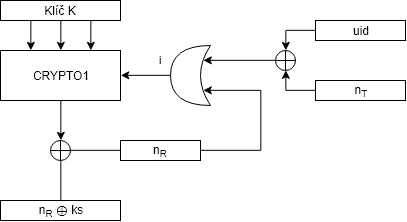
\includegraphics[width=0.7\linewidth]{obrazky-figures/cryptoInitialization.png}\\[1pt]  
  \caption{Diagram inicializace šifry CRYPTO1, kde ks je šifrovací proud (keystream)\cite{Dismantling_Mifare_Classic}}    
  \label{obrazekInicializaceSifry}
\end{figure*}

\subsection{Autentizace}
\label{autentizace}
Komunikace karet Mifare Classic implementuje standard ISO~14443. Ve čtvrté části se implementace od standardu liší a Mifare zde používá svůj vlastní, neveřejný protokol. Po vstupu do blízkosti čtecího zařízení a nabití karty nastává antikolizní fáze (viz~\ref{obrazekZacatekKomunikace}). Komunikaci zahajuje čtecí zařízení příkazem Select. Odešle \emph{0x93 20}, na což karta odpoví svým~UID~\emph{u}. Čtecí zařízení pošle \emph{0x93~70} následováno~UID vybrané karty a dvěma byty~CRC. Antikolizní fáze je ukončena odpovědí karty~SAK (z anglického Select acknowledge). Nyní je karta v aktivním stavu a připravena přijímat příkazy vyšší vrstvy\cite{PracticalAttackOnMifare}.
\par
Čtecí zařízení požádá o autentizaci pro specifický blok odesláním požadavku \emph{0x~60~00~F5~7B}. První byte \emph{0x60} znamená, že se má autentizace provést s klíčem A. Pro autentizaci s klíčem B musí být byte \emph{0x61}. Druhým bytem se vybere blok, pro který se chce čtecí zařízení autentizovat. Blok~0 je v sektoru~0, autentizace tedy proběhne pro celý sektor~0. Pokud by byl požadován například blok~5, autentizace proběhne pro sektor~1. Zbývající dva byty jsou opět CRC\cite{PracticalAttackOnMifare}. 
\par
Na tento požadavek karta pošle výzvu (anglicky challenge)~${n_T}$\footnotemark ve formě takzvané nonce\cite{Wirelessly_Pickpocketing}. Nonce je anglický výraz pro slovo na jedno použití. V kryptografii označuje náhodné číslo použité při komunikaci pouze jednou\cite{Nonce_Based_Encryption}. Od této chvíle je komunikace šifrována, tedy XORována s pseudonáhodným proudem bitů (anglicky keystream). Čtecí zařízení odpoví se svou vlastní výzvou~${n_R}$ a odpovědí na výzvu karty~${a_R = suc^{64}(n_T)}$. Autentizace je dokončena odpovědí karty~${a_T = suc^{96}(n_R)}$. Po této odpovědi jsou karta i čtecí zařízení vůči sobě autentizovány. Autentizace je platná pouze pro sektor, o který bylo požádáno\cite{Wirelessly_Pickpocketing}. 

\footnotetext{Notace je zachována stejná jako v \cite{Wirelessly_Pickpocketing}, tedy \emph{T} jako tag, \emph{R} jako reader, \emph{n} jako nonce a \emph{a} jako answer}

\begin{figure*}[ht]\centering
  \centering
  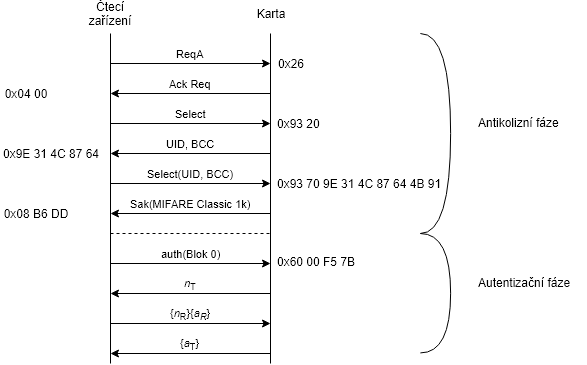
\includegraphics[width=\linewidth]{obrazky-figures/commDiagram.png}\\[1pt]  
  \caption{Antikolizní a autentizační fáze komunikace. Šifrované zprávy jsou ve složených závorkách.\cite{Dismantling_Mifare_Classic}}    
  \label{obrazekZacatekKomunikace}
\end{figure*}

\subsection{Komunikační protokol}
\label{komunikacni_protokol}
\par
Pro manipulaci s daty mají karty Classic malou sadu příkazů. Aby mohly být provedeny nad datovým blokem, musí být čtecí zařízení autentizováno pro sektor, který tento blok obsahuje. Před každým použitím jakéhokoliv příkazu se kontrolují přístupové podmínky. Ne všechny příkazy mohou být povoleny. Například blok může být nastaven pouze pro čtení nebo jiný blok s hodnotou může být pouze inkrementován\cite{PracticalAttackOnMifare}.\par
Po autentizaci následuje šifrovaná komunikace s kartou. Příkazy Read a Write čtou či zapisují jeden blok. Ten může být jak datový, tak hodnotový. Příkaz Write může být použit k formátování datového bloku na blok s hodnotou nebo na zapsání libovolných dat do bloku. Další příkazy jsou povoleny pouze na hodnotových blocích. Jsou to Decrement, Increment, Restore a Transfer. Příkazy Increment a Decrement inkrementují nebo dekrementují hodnotu hodnotového bloku a výsledek vloží do paměťového registru. Příkaz Restore načte do registru hodnotu nezměněnou a příkaz Transfer nahraje hodnotu z registru zpět do stejného nebo jiného bloku\cite{PracticalAttackOnMifare}.

\chapter{Známé zranitelnosti}
\label{zranitelnosti}
Zabezpečení není silnou stránkou karet Mifare Classic. Tato podkapitola obsahuje popis jednotlivých nedostatků. Nedostatečná délka šifrovacích klíčů je první z nich. Následuje předvídatelnost výzev posílaných při autentizaci. Popsáno je také nedostatečné řešení výpočtu paritních bitů. Další zranitelnosti jsou více kryptografického rázu, s jejichž pomocí lze získat aktuální stav šifry a vrátit ho do stavu, kdy obsahoval tajný klíč sektoru. Nakonec je popsána zranitelnost při autentizaci více sektorů, která byla pojmenována jako vnořená autentizace.
\par
\section{Krátké šifrovací klíče}
Pro šifrování karet se používají 48bitové klíče. Tato délka klíčů je ale příliš malá na to, aby zabránila úspěšnému brute force útoku v dosažitelném čase. Proto bylo zavedeno zpoždění v komunikaci a v autentizaci. Každý pokus by trval 6 milisekund. Díky této kompenzaci by online brute force útok na jeden sektor, prohledávající všech $2^{48}$ možných klíčů, trval více než 44~tisíc let. Odhalení algoritmu šifry CRYPTO1 umožnilo provést offline brute force útok. V takovém případě útočník nemusí komunikovat se zařízením pod útokem. Stačí mu pouze záznam komunikace, tím se eliminuje zavedené zpoždění. V prosinci 2007 Nohl a Plötz uvedli, že zařízení za 100\$ dokáže najít klíč přibližně za týden. Tato doba lze dál zkrátit přidáním paměti\cite{Cryptanalisis}.
\par
\section{Předvídatelné výzvy}
\label{predvidatelne_nonce}
Aby mohly kryptografické protokoly poskytovat správné zabezpečení, je pro ně zásadní dostatečný generátor pseudonáhodných čísel. Čísla pro Mifare Classic generuje 16bitový LFSR. Výzvy $n_T$ (nonce, viz. \ref{komunikacni_protokol}) použité při autentizaci jsou ale 32bitové. To znamená, že první polovina $n_T$ určuje její zbytek. Sekvence všech výzev se opakuje každých $2^{16} - 1$ cyklů\cite{Cryptanalisis}. Cyklus generátoru karty je rozdílný od čtecího zařízení. Zatímco karta mění stav každou periodu hodinového signálu, čtecí zařízení aktualizuje stav jen při volání generátoru\cite{Dismantling_Mifare_Classic}. Generátor v kartě se resetuje do původního stavu při každém nastartování karty. Výzva poslaná kartou je tedy podmíněna pouze časem mezi zapnutím elektromagnetického pole k nabití karty a momentem odeslání žádosti o autentizaci. Autentizace je tedy zbavena jakékoliv náhodnosti. \par
Útočník s fyzickým přístupem ke kartě ji může ''přinutit'' k odeslání vždy stejné výzvy. K tomu je potřeba po každém pokusu vypnout elektromagnetické pole (zhruba na 30$\mu$s), aby se vybily všechny kondenzátory, znovu zapnout pole a počkat konstantní čas před odesláním požadavku o autentizaci. Druhý způsob spočívá v čekání mezi opětovným odesláním požadavku přesně stanovený čas \emph{t}. Stav generátoru pseudonáhodných čísel se mění každých 9,44$\mu$s. Na vystřídání všech stavů tak stačí pouze $(2^{16} - 1) * 9,44\mu$s $= 618,650ms$. Velikost výzvy je dvojnásobná oproti LFSR, výsledný čas \emph{t} je tedy poloviční $t = 618,650ms/2 = 309,325ms$ \cite{Wirelessly_Pickpocketing}. V novější verzi karet Classic EV1 je tento nedostatek odstraněn nahrazením generátoru pseudonáhodných čísel generátorem náhodných čísel\cite{Mifare_Classic_Official_about}.

\section{Paritní bity}
\label{paritni_bity}
Další slabinou karet Mifare Classic je jejich řešení paritních bitů. Podle standardu ISO~14443 musí každý odeslaný byte následovat lichý paritní bit. Karty Classic sice s každým odeslaným bytem posílají paritní bit, ten je ale vypočítán už z důvěrného textu (plaintext) a ne z textu šifrovaného (ciphertext), který je skutečně posílán komunikační vrstvou. Kromě toho odeslané paritní bity jsou šifrovány stejným šifrovacím bitem (keystream), který je použit pro šifrování dalšího bitu plaintextu (viz \ref{parityDiagram})\cite{Cryptanalisis}.
Kvůli tomu je s každým odeslaným bytem vyzrazena jednobitová informace o důvěrném textu\cite{Dismantling_Mifare_Classic}. 
\begin{figure*}[ht]\centering
  \centering
  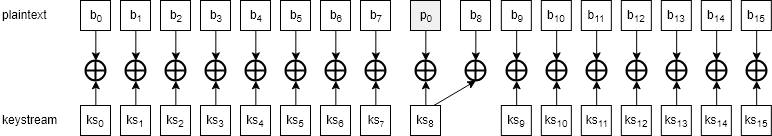
\includegraphics[width=\linewidth]{obrazky-figures/parityBits.png}\\[1pt]  
  \caption{Šifrování paritních bitů \cite{Cryptanalisis}}   
  \label{parityDiagram}
\end{figure*}
\par
V souvislosti s paritními bity existuje ještě jedna slabina. V průběhu autentizační fáze karta vždy nejprve kontroluje právě paritní bity. Když karta přijme $\{n_R\}\{a_R\}$ (viz. \ref{autentizace}) a nějaký z osmi paritních bitů je špatný, karta neodešle žádnou odpověď. V případě že jsou všechny paritní bity správné, ale $a_R$ je špatně, karta odešle 4bitovou chybovou zprávu $0x5$ indikující selhání autentizace. Jak bylo řečeno v \ref{autentizace}, komunikace je v tuto chvíli šifrována. I~když se čtecí zařízení úspěšně neautentizovalo, dostane chybovou zprávu zašifrovanou. Nelze předpokládat, že si ji správně rozšifruje a dozví se, že došlo k selhání.
Jelikož je kód této chyby známý, lze z šifrované zprávy získat 4 bity keystreamu. Přestože se takovýto únik nemusí zdát jako velký problém, je nepostradatelnou částí mnoha útoků, které cílí na klíče těchto karet.
\par
Jestliže se čtecí zařízení nemá jak dozvědět o selhání při autentizaci, pak nezáleží na tom, jestli dostane zprávu šifrovanou nebo žádnou. Zmíněná slabina tedy lze odstranit vydáním nových karet, které při autentizaci neposílají žádné chybové kódy. Tato metoda je sice nákladná pro již zavedené systémy s kartami v oběhu, ale je pořád kompatibilní s Mifare Classic protokolem\cite{Cryptanalisis}. 

\section{Navrácení stavu posuvného registru}
Stav posuvného registru na začátku inicializace obsahuje tajný klíč sektoru. V průběhu autentizace a šifrování se stav tohoto registru mění. Pokud by se útočníkovi podařil nějakým způsobem získat stav registru v určitém čase a záznam komunikace, lze jednotlivé změny stavu obrátit a deterministicky spočítat jakýkoliv předchozí stav registru včetně tajného klíče.\cite{Dismantling_Mifare_Classic} 

\section{Získání stavu šifry}
Pro získání aktuálního stavu registru v CRYPTO1 existují dvě metody. První metoda využívá výzev manipulujících se stavem šifry při autentizaci. Nejprve je potřeba vygenerovat tabulku dvojic (\emph{lfsr}, \emph{ks}), kde \emph{lfsr} jsou stavy registru určitého formátu (\emph{0x000WWWWWWWWW}) a~\emph{ks}~je prvních 64 bitů keystreamu. Předpočítaná tabulka je~znovupoužitelná na jakýkoliv klíč/čtecí zařízení. Výsledek obsahuje $2^{36}$~dvojic zabírající přibližně 1TB. Následuje útok na samotné čtecí zařízení. Pro každý stav 0xXXX je zahájena autentizace se zafixovaným UID karty a výzvou karty ve tvaru $n_T = 0x0000XXX0$. Po odpovědi čtecího zařízení ve tvaru $n_R \oplus ks_1, suc(n_T) \oplus ks_2$ se v~komunikaci nepokračuje. Na to většina čtecích zařízení odešle~$halt \oplus ks_3$(tento útok lze provést i nad čtecími zařízeními, které příkaz halt neodešlou). Protože $suc(n_T)$ a formát příkazu halt jsou známé, je možné získat i $ks_2$ a $ks_3$. Existuje právě jedna hodnota~0xXXX, která změní stav šifry do jednoho ze stavů v předpočítané tabulce. Tento stav odhalíme vyhledáním $ks_2, ks_3$ v tabulce. V konfiguraci této metody lze vyměnit paměť za čas, tedy místo 12 bitů měnit bitů 13, snížit velikost tabulky na polovinu, ale zdvojnásobit počet potřebných autentizací.\cite{Dismantling_Mifare_Classic}
\par
Druhá metoda využívá chyby v návrhu filtrační funkce \ref{filterFunction}. Konkrétně toho, že její vstupy jsou pouze na lichých pozicích registru. Vstupním požadavkem je část keystreamu. Bity LFSR použité při výpočtu sudých a lichých bitů keystreamu lze generovat odděleně. Rozdělením také zpětné vazby na dvě části lze zkombinovat tyto sudé a liché části, čímž vzniknou právě ty stavy LFSR, které generují daný keystream.\cite{Dismantling_Mifare_Classic}

\section{Vnořená autentizace}
Za předpokladu, že útočník zná některý z tajných klíčů a je jím ověřen vůči příslušnému bloku karty, autentizace vůči dalším blokům probíhá trochu jinak než při první autentizaci. Další autentizaci zahájí útočník odesláním požadavku o autentizaci. Tento požadavek je šifrovanán původním klíčem předchozího bloku, narozdíl od první autentizace, kdy požadavek nebyl šifrován vůbec. Po zpracování požadavku je vnitřní stav šifry CRYPTO1 nastaven na klíč nového sektoru a autentizační protokol popsaný v \ref{autentizace} začíná od začátku (ovšem bez antikolizní fáze). Změna nastává při odesílání výzvy $n_T$. Ta je totiž nyní odeslána zašifrovaná s tím, že pro šifrování byl použit již nový klíč. Se znalostí šifrování paritních bitů z \ref{paritni_bity} je možné zredukovat $2^{16}$ výzev na pouhých 64. Kvůli implementaci slabého pseudonáhodného generátoru čísel lze téměř s jistotou určit, která výzva je ta správná. Odeslaná výzva závisí na takzvané vzdálenosti od předchozího pokusu o autentizaci. Tato vzdálenost byla popsána v \cite{Dismantling_Mifare_Classic} jako počet posunutí registru generátoru čísel. Pomocí odhadnuté výzvy lze odhalit 32 bitů šifrovacích bitů (keystream)\cite{Dismantling_Mifare_Classic}.
Tuto slabinu využívají například útoky popsané v \cite{Cryptanalisis} a v \cite{Wirelessly_Pickpocketing} kde je útok nazván vnořeným útokem (nested attack).

%                               NADPIS                      
\chapter{Chameleon Mini}
\label{chameleon_mini}
V této kapitole bude představeno zařízení Chameleon Mini, jeho původ, využití, hardware a výběr podporovaných příkazů.
\par

Chameleon Mini je zařízení velikosti běžné kreditní karty německé firmy Kasper \& Oswald. Zařízení je navrženo jako univerzální nástroj pro praktickou bezpečnostní analýzu NFC\footnotemark a RFID systémů, penetrační testování nebo různé jiné aplikace koncových uživatelů. Tato volně programovatelná platforma umožňuje emulovat existující komerční chytré karty, a to včetně kryptografických funkcí a unikátních identifikátorů (UID). Dále může být využito v různých scénářích útoků, na odposlech NFC a RFID komunikace nebo funkční testování RFID vybavení. O bezstarostné nahrávání firmware se stará USB zavaděč. Pomocí praktické a lehce zapamatovatelné příkazové sady lze měnit nastavení a chování zařízení. Zároveň dokáže do vnitřní paměti uložit a virtualizovat až osm bezkontaktních karet.\cite{ChameleonKickStarter} 
\footnotetext{z anglického {Near-field} communication}
\par 
Projekt Chameleon Mini byl založen na Porúrské univerzitě v Bochumi a je financován pomocí crowdfundingu na platformě KickStarter. V současné době se veškerý oficiální firmware, schémata tištěných spojů nebo podpůrné nástroje nachází v {open-source} repozitáři služby GitHub\footnotemark.\cite{ChameleonDocs}
\footnotetext{\url{https://github.com/emsec/ChameleonMini}}

\section{Hardware}
Zařízení je prodáváno jako deska plošných spojů. Nejnápadnější částí je pak anténa schopná generovat RFID pole o frekvenci 13,56MHz. Chameleon Mini může emulovat karty standardů ISO 14443, ISO 15693, NFC tagy a díky RFID poli dokáže vystupovat také jako aktivní čtecí zařízení.\cite{ChameleonKickStarter} Dosah antény je závislý na módu zařízení. Při emulaci karet má na dosah vliv také typ čtecího zařízení. V tomto případě se tak dosah pohybuje od 0 do 8,5cm. Dosah v módu čtecího zařízení závisí na tvaru a typu čteného tagu. Standardní bezkontaktní karty lze číst na vzdálenost 1,5cm. Malé tagy (například Mifare UltraLight) je potřeba položit přímo na anténu.\cite{ChameleonEshop} Pro praktické a bezdrátové použití lze pomocí USB nabít {lithium-iontovou} baterii přímo na desce. Po plném nabití je možné zařízení používat zhruba hodinu. Interakci v bezdrátovém módu umožňují dvě integrovaná, nastavitelná tlačítka a LED diody. Baterii je možné odpojit pomocí vypínače a šetřit tak její energii. Pomocnými piny lze připojit jakékoliv externí vybavení a zakomponovat tak možnosti tohoto nástroje například do zámku dveří nebo jiného zařízení IoT (z anglického Internet of Things, internet věcí).\cite{ChameleonKickStarter}
\par
Vnitřní logiku po hardware stránce zajišťuje mikrokontroler Atmel ATXMega128A4U. Ten poskytuje funkce pro {radio-frekvenční} kódování a dekódování, rozhraní USB a je v něm nahraný stavový automat, kterým je řízen chod zařízení. Mikrokontroler obsahuje podporu AES a DES na hardware úrovni. Výpočty těchto kryptografických algoritmů jsou tak podle výrobce až třikrát rychlejší než na originálních kartách (Mifare DESfire). Jako operační paměť slouží 128kB Flash paměť, 2kB EEPROM paměť a 8kB SRAM paměť. Do volatilní paměti SRAM je ukládána odposlouchaná komunikace. Tu je možné zapsat do nevolatilní 128kb FRAM paměti, která slouží také jako uložiště pro virtuální karty.\cite{ChameleonKickStarter}

\section{Podporované příkazy}
Ke komunikaci se zařízením Chameleon Mini lze použít příkazovou řádku, emulátor terminálu nebo vlastní skripty a aplikace. Struktura firmware umožňuje jednoduchou rozšiřitelnost o nové, nepodporované standardy a karty. Tlačítkům a LED diodám je možné přiřadit různé funkce. Přenos dat mezi zařízením a počítačem přes USB zajišťuje protokol {X-MODEM}. \cite{ChameleonKickStarter}
\par
Chameleon Mini připojený pomocí USB do počítače je zobrazeno jako sériové zařízení. Zařízení se nastavuje a ovládá příkazy posílanými přes rozhraní příkazové řádky. K tomuto rozhraní jsem přistupoval pomocí programu Putty. Příkazy je možné použít se čtyřmi různými syntaxemi.
\begin{itemize}
  \item <Příkaz>=<Hodnota> Nastaví parametr zařízení
  \item <Příkaz>=? Vypíše seznam všech možných hodnot parametru
  \item <Příkaz>? Vrátí aktuální hodnotu parametru
  \item <Příkaz> Provede funkci a vypíše možnou odpověď
\end{itemize}
Chameleon poskytuje osm slotů, které je možno nakonfigurovat jako aktivní čtecí zařízení, pasivní zařízení pro odposlech komunikace (sniffing) nebo pro uložení různých virtualizovaných karet. V každém slotu je uložena jeho konfigurace a případně obsah karty. Číslo právě aktivního slotu zjistí příkaz \verb|Setting?|. Jiný slot aktivujeme pomocí \verb|Setting=X|, kde \emph{X} je číslo od 1 do 8. Příkaz \verb|Config?| vrátí konfiguraci aktivního slotu. Všechny možné konfigurace vyjmenuje \verb|Config=?| a opět změnu konfigurace například na emulaci karty Mifare Classic provede příkaz \verb|Config=MF_CLASSIC_1K|(viz. část \ref{komunikaceChameleon}). \par 
Každý odeslaný příkaz následuje odpověď zařízení s číslem a zprávou stavu. První cifra třímístného čísla stavu ukazuje vážnost odpovědi. Zprávy s číslem začínající cifrou ''1'' jsou spíše informačního charakteru, zatímco cifra ''2'' značí chybu.\cite{ChameleonDocs}

\begin{lstlisting}[caption=Záznam komunikace se zařízením Chameleon Mini, label={komunikaceChameleon}]
Setting?
101:OK WITH TEXT
2
Setting=4
100:OK
Config?
101:OK WITH TEXT
NONE
Config=?
101:OK WITH TEXT
NONE,MF_ULTRALIGHT,MF_ULTRALIGHT_EV1_80B,MF_ULTRALIGHT_EV1_164B,MF_CLASSIC_1K,
MF_CLASSIC_1K_7B,MF_CLASSIC_4K,MF_CLASSIC_4K_7B,ISO14443A_SNIFF,
ISO14443A_READER
Config=MF_CLASSIC_1K
100:OK
\end{lstlisting}

Slotu s konfigurací virtualizace karty můžeme nastavit libovolné UID příkazem \verb|UID=<UID>|. Stejně jako v předchozím případě neznámé UID zjistíme voláním \verb|UID?|. V některých případech je potřeba nastavit náhodné UID virtualizované karty, například jako opatření proti ukládání škodlivých UID na černou listinu. Toho lze docílit nastavením jednoho z tlačítek \verb|Rbutton=UID_Random| jeho zmáčknutím. V rozhraní příkazové řádky tato funkce (zatím) zveřejněná není, ale pomocí tlačítka lze UID měnit přímo v terénu bez připojení k počítači.\par
Při komunikaci může dojít ke změně paměti virtualizované karty, například snížení kreditu na kartě. Obnovením paměti karty by se kredit dostal do původního stavu a šel by znovu použít. Voláním příkazu \verb|Store| se aktuální stav karty uloží z FRAM do paměti nevolatilní paměti Flash. Po domnělé změně stavu karty \verb|Recall| načte kartu zpět do FRAM, připravenou k použití v původním stavu. Tato funkcionalita lze provázat s dvěma tlačítky na zařízení příkazy \verb|Rbutton=Store_Mem|, respektive \verb|Rbutton=Recall_Mem|.\par
Voláním příkazu \verb|Download| je možné stáhnout obraz karty ze zařízení. Samotný přenos začne po navázání spojení protokolem {X-Modem}. Připojení tímto protokolem podporuje například program Tera Term. Mimo to se obraz karty dá stáhnout pomocí programu Chameleon Mini GUI\footnotemark, který poskytuje přehledné grafické rozhraní pro manipulaci se zařízením. Stažený obraz karty do aktivního slotu zařízení načte příkaz \verb|Upload|, který opět počká na připojení {X-Modem}. Příkazem \verb|Clear| se smaže celý obsah karty aktivního slotu.\par
\footnotetext{\url{https://github.com/iceman1001/ChameleonMini-rebootedGUI}}
Chameleon Mini v módu čtecího zařízení nabízí trochu jinou funkcionalitu, a tedy i jiné příkazy než v módu virtualizace karet. Mód čtecího zařízení aktivuje příkaz \\\verb|Config=ISO14443A_READER|. Tento mód je aktivován nad aktivním slotem. Jakákoli data v tomto slotu jsou smazána. Tato konfigurace slotu neovlivňuje jiné sloty. Je tedy možné mít například první slot čtecí a ostatní emulující různé karty. \par
Základní příkaz této konfigurace je \verb|Send| případně \verb|Send_Raw|, které slouží k odesílání dat kartě. Příkaz \verb|Send|, pokud je parametr delší než jeden byte, přidá paritní bity a odešle zprávu. Naopak příkaz \verb|Send_Raw| předpokládá, že paritní bity jsou v parametru zprávy už obsaženy a odešle ji rovnou. Oba příkazy mohou mít jeden nebo dva parametry. Parametry jsou odděleny mezerou a nejsou uzavřeny v žádných závorkách. Jedním parametrem je předána zpráva k odeslání ve formě hexadecimálního čísla. V případě dvou parametrů je zpráva až druhý parametr. Prvním je předán počet bitů k odeslání opět ve tvaru hexadecimálního čísla. Po odeslání zprávy zařízení chvíli počká na odpověď a pokud ji přijme, zbaví ji paritních bitů a na příkazovou řádku vytiskne přijatou zprávu, její délku v bitech a buď \emph{PARITY OK}, nebo \emph{PARITY ERR} v závislosti na výsledku kontroly parity. Pokud žádnou odpověď neobdrží, vrátí \emph{NO DATA}.\par
Jelikož čtecí zařízení je aktivní prvek, poskytuje Chameleon Mini možnost ovládat jeho elektromagnetické pole. Za pomoci příkazu \verb|Field=1| lze toto pole zapnout. Naopak příkaz \verb|Field=0| pole vypne. Aktuální stav zjistí \verb|Field?|.\par
Jak již bylo zmíněno, pro interakci s uživatelem jsou na zařízení dvě konfigurovatelná tlačítka, levé a pravé. Kromě toho Chameleon rozlišuje mezi dlouhým a krátkým stiskem tlačítek, kdy stisk tlačítka delší než $1.28ms$ značí dlouhý stisk. Dohromady jsou tedy čtyři konfigurační příkazy těchto tlačítek, a to:
\begin{itemize}
\item Lbutton
\item Rbutton
\item {Lbutton\_Long}
\item {Rbutton\_Long}
\end{itemize}
Každý z těchto příkazů podporuje nastavení (''=''), získání aktuálního stavu (''?'') a nápovědu (''=?''). \par
Stav zařízení v terénu lze zjišťovat dvěma LED diodami, které se nastavují příkazy \verb|Ledred| a \verb|Ledgreen|. Diody mohou indikovat například změnu a stav paměti, komunikaci s terminálem nebo přítomnost elektromagnetického pole čtecího zařízení. Je jen na uživateli, jak diody nastaví.\cite{ChameleonDocs}

    
    \chapter{Testovací prostředí a podpůrné nástroje}
Tato kapitola se věnuje testovacímu prostředí, ve kterém budou demonstrovany vybrané zranitelnosti. Některé demonstrace vyžadují implementační část. Pro usnadnění práce byla implementována knihovna tříd. Dokumentace její implementace je také součástí této kapitoly.

\section{Testovací prostředí}
Testování vybraných zranitelností probíhalo v reálném prostředí na čtecím zařízení HID RP10\footnotemark. Po přiložení osobní karty studenta, či učitele je možné otevřít dveře a vstoupit. Karty používané studenty jsou mezinárodní studentské ISIC karty, případně VUT karty. Tyto karty jsou typu Mifare Classic, a jsou tedy vhodné k těmto demonstracím. Testování implementovaných demonstrací probíhalo na operačním systému Windows 10 Pro. Při testování byla použita zařízení Chameleon Mini, popsaná v kapitole \ref{chameleon_mini}.\par
\footnotetext{\url{https://www.sourcesecurity.com/hid-rp10-access-control-reader-technical-details.html}}


\section{Implementace modulů}
\label{implementaceModulu}
První a poslední demonstrace vyžadují programovou implementaci. Nejdříve byly implementovány takzvané moduly, tedy třídy abstrahující komunikaci se zařízením Chameleon Mini nebo poskytující pomocné funkce. Všechny moduly jsou zapouzdřeny v knihovně tříd \verb|MifareModules|. Některé z modulů mají vlastnost \verb|Verbose| typu \verb|Boolean|. Jejím nastavením na \verb|true| začnou moduly zapisovat aktuální stav na standardní výstup k ulehčení ladění. Celá programová část této práce byla realizována v jazyce C\# .Net Framework verze 4.6.

\subsection*{SerialModule}
Třída \verb|SerialModule| pozměňuje funkcionalitu \verb|System.IO.Ports.SerialPort| (dále jen \\\verb|SerialPort|) tak, aby vyhovoval požadavkům modulů vyšší vrstvy. V parametru konstruktoru je předávána třída \verb|SerialModuleConfig|, která obsahuje veškeré možné nastavení komunikace přes sériový port. Třída je předpřipravená tak, že beze změn zajišťuje komunikaci se zařízením Chameleon Mini na portu ''COM3''. Konstruktor vytvoří komponentu \verb|SerialPort| se zadanou konfigurací a rovnou jej otevře pro komunikaci.

\begin{lstlisting}[caption=Metody třídy \emph{SerialModule}, label={serialModuleMethods}]
public SerialModule(SerialModuleConfig config)
public void Open()
public void Close()
public void WriteLine(string message)
public string ReadLine()
public List<string> ReadLines(int numberOfLines)
public List<string> WriteAndGetResult(string message, int numberOfLines = 1)
public void WriteAndTrashResult(string message, int numberOfLines = 1)
\end{lstlisting}

Práce metod \verb|Open()|, \verb|Close()|, \verb|WriteLine(string)| a \verb|ReadLine()| je vcelku jednoznačná. První dvě se starají o otevírání, respektive zavírání portu pro komunikaci. Pomocí třetí metody lze zapsat řetězec na otevřený port a poslední metoda řetězec z portu přečte. Tyto dvě metody mohou zapisovat řetězce komunikace na standardní výstup. Metoda \verb|ReadLines(int)| přečte z portu několik řádků, v závislosti na jejím parametru a vrátí je jako seznam řetězců. Poslední dvě metody zjednodušují zápis a následné zpracování odpovědi. Metoda \verb|WriteAndGetResult(string, int)| odešle zprávu a vrátí řádky odpovědi opět jako seznam řetězců. Není možné předpovědět, kolik řádků bude odpověď mít, proto je nutné zadat počet řádků k přečtení. Při zadání většího čísla než je počet řádků, metoda vrátí všechny řádky, které přečetla, a po zachycení vyjímky \verb|TimeoutException| skončí. Zadáním menšího čísla metoda přečte a vrátí daný počet řádků. Problém nastane při dalším čtení, kdy nepřečtené řádky zůstanou ve vyrovnávací paměti portu a budou přečteny místo nových. Poslední metoda \verb|WriteAndTrashResult(string, int)| funguje stejně jako předchozí metoda s tím rozdílem, že přečte odpověď, ale už ji nevrátí.

\subsection*{ChameleonModule}
Tento modul abstrahuje komunikaci se zařízením Chameleon Mini tak, aby se uživatel nemusel starat o obsluhu sériového portu. Konstruktory jsou dva. Prvním je v parametru předána pouze instance třídy \verb|SerialModule|. Tímto způsobem je předána informace, na kterém portu zařízení komunikuje. Druhým konstruktorem lze navíc specifikovat roli zařízení (při relay útoku) kvůli zápisu informací do konzole.

\begin{lstlisting}[caption=Metody třídy \emph{ChameleonModule}, label={chameleonModuleMethods}]
public ChameleonModule(SerialModule serial)
public ChameleonModule(SerialModule serial, string role)
public void GetCommands()
public void Send(string message)
public List<string> ReadToEnd()
public string SendWithAnswer(string message)
public string GetUid()
public void TurnElectromagnetic(Field value)
private string CalculateMessageLength(string message)
\end{lstlisting}

Metoda \verb|GetCommand()| je spíše informativního charakteru a vrátí všechny příkazy, které Chameleon podporuje. Pomocí metody \verb|Send(string)| se odešle zpráva ve formátu hexadecimálního čísla v řetězci. Metoda sama vypočítá délku zprávy a připojí ji k příkazu \verb|Send| pro Chameleon Mini. Metoda \verb|ReadToEnd()| přečte všechny řádky odpovědi po příkazu \verb|Send|. V této části už je známý počet řádků, jelikož všechny odpovědi končí buď řádkem ''PARITY OK'', ''PARITY ERR'', nebo ''NO DATA''. Funkcionalitu obou předchozích metod kombinuje \verb|SendWithAnswer(string)|. Tato metoda odešle zadanou zprávu a vrátí relevantní část odpovědi. Pokud se v blízkosti zařízení nachází kompatibilní karta, metodou \verb|GetUid()| získáme její UID. Elektromagnetické pole zařízení ovládá poslední veřejná metoda \\\verb|TurnElectromagnetic(Field)|. Ta má jako parametr výčtový typ \verb|Field| s hodnotami ''Off'' a ''On''. Poslední významná metoda je privátní \verb|CalculateMessageLength(string)|, jenž vypočítá již zmíněnou délku zprávy k odeslání. 

\subsection*{CardModule}
Poslední z komunikačních modulů je zaměřen na komunikaci  přímo s kartou a obsahuje metody usnadňující práci s protokolem ISO 14443. Informaci o tom, u kterého zařízení se karta nachází, je jedinému konstruktoru předána parametrem typu \verb|ChameleonModule|. Tato třída dále závisí na \verb|CRCModule|, ten se ale parametrem nepředává. Jeho instance je vytvořena v konstruktoru. Třída však pokrývá pouze antikolizní fázi a začátek autentizační fáze. Pro další by byly potřebné knihovny s šifrou CRYPTO1. 
\begin{lstlisting}[caption=Metody třídy \emph{CardModule}, label={cardModuleMethods}]
public CardModule(ChameleonModule cm)
public string ReqA()
public string Select()
public string SelectUid(string uid)
public string AuthenticateForBlock(string blockNumber)
private string Get(ISOCode code)
\end{lstlisting}

Antikolizní fáze protokolu ISO~14443 je inicializována metodou \verb|ReqA()|. Metoda \verb|Select()| odešle příkaz \emph{Select} podle protokolu a pomocí metody \verb|SelectUid(string)| je vybrána karta na základě jejího UID. Po této sekvenci je antikolizní fáze. Metoda \\\verb|AuthenticateForBlock(string)| začne s autentizační fází vůči paměťovému bloku na kartě. Vybraný blok je zadán ve formě řetězce hexadecimálního čísla. Všechny metody ke zprávám připojují kódy protokolu ISO~14443 nebo případně kontrolní součty CRC. Každá z těchto metod vrací odpovědi karty. Nedílnou součástí tohoto modulu je výčtový typ \verb|ISOCode| s hodnotami kódů standardu. Čísla kódů z výčtového typu získává privátní metoda \verb|Get(ISOCode)|.

\subsection*{CRCModule}
Třída tohoto modulu zapouzdřuje a zjednodušuje použití externí knihovny \\\verb|Nito.KitchenSink.CRC|\footnotemark, která slouží pro výpočet kontrolních součtů CRC. Konstruktor vytvoří instanci třídy \verb|CRC16| se správným nastavením pro použití v předchozím modulu. Jediná metoda třídy \verb|Hash(string)| vypočítá a vrátí kontrolní součet zadané hodnoty. 

\footnotetext{\url{https://www.nuget.org/packages/Nito.KitchenSink.CRC/}}

\chapter{Demonstrace vybraných zranitelností}
Tato kapitola se věnuje návrhu, implementaci, provedení a vyhodnocení tří vybraných zranitelností karet Mifare Classic. Nejprve se zaměřím na analýzu předvídatelných výzev karty Mifare Classic popsaných v části \ref{predvidatelne_nonce}. Následují možnosti a úskalí emulace karet pomocí zařízení Chameleon Mini. Nakonec nastíním princip a provedení relay útoku.\par 

\section{Časová krypto-analýza}
\label{casovaKryptoanalyza}
Jako první demonstraci jsem vybral zranitelnost nedostatečné náhodnosti generování výzev karty ve fázi autentizace, popsané v části \ref{predvidatelne_nonce}. Tato analýza se týká pouze karet, protože generátor pseudonáhodný čísel ve čtecích zařízeních funguje jiným způsobem. Karty Mifare Classic generují 32bitové výzvy 16bitovým posuvným registrem s lineární zpětnou vazbou, jehož stav se mění každou periodu hodinového signálu karty a při startu karty se jeho stav resetuje vždy do stejného stavu. Perioda hodinového signálu je 9,44$\mu$s, zatímco perioda generátoru pseudonáhodných čísel je 65535. Generátor tedy vyčerpá všechny stavy během přibližně 0,618s. Odesláním požadavku o autentizaci vždy ve správný čas docílíme téměř konstantní výzvy karty. \par
S těmito znalostmi můžeme navrhnout dva způsoby, jak si kartou nechat vygenerovat vždy stejnou výzvu. První možností je mezi každým požadavkem o autentizaci čekat stanovený čas. Tímto počkáme až proběhne perioda generátoru pseudonáhodných čísel a jeho stav se bude rovnat stavu v době předchozího pokusu. Druhou možností je odesílat pokusy o autentizaci vždy ve stejný čas od startu karty. Startem karty se generátor pseudonáhodných čísel resetuje do konstantního stavu. Vyčkáním generátor vygeneruje vždy stejnou výzvu.\par
První možnost je z hlediska času náročnější. Aby bylo dosaženo požadovaného výsledku, musejí být žádosti odesílány pouze každých 0,618s. Naopak pokusy v druhé možnosti lze opakovat téměř ihned po získání výzvy. Za stejnou dobu tak lze získat větší množství výzev k porovnání. Využitím příkazu \verb|Field| zařízení Chameleon Mini můžeme ovládat stav elektromagnetického pole zařízení a tím start karty. K analýze této zranitelnosti tak bude využita druhá možnost.\par
Cílem této demonstrace je ověřit možnost získání stejných výzev s vysokou pravděpodobností za pomoci zařízení Chameleon Mini. Výzva karty je použita jako jedna ze složek vstupního bitu použitého při inicializaci šifry CRYPTO1 (viz část \ref{crypto1section}). Ovládáním výzvy karty útočník ovládne celý inicializační proces šifry karty, a tím i šifrovací bity použité k šifrování důvěrného textu. \par
\subsection{Implementace}
Tato demonstrace vyžaduje implementaci skriptu či programu, který automatizuje obsluhu elektromagnetického pole a průběh antikolizní a autentizační fáze. Chameleon v tomto případě napodobuje čtecí zařízení, bude tedy nastaven do konfigurace \verb|ISO14443A_READER|. Při demonstraci bude Chameleon Mini opakovaně zapínat a vypínat své elektromagnetické pole a mezi tím vždy proběhne požadavek o autentizaci s kartou. Karta odešle výzvu, ta se uloží do seznamu a cyklus začíná od znova. Nakonec bude seznam výzev prohledán na duplikáty.\par
Program \emph{CryptoAnalysis.exe} využívá knihovny \verb|MifareModules| (viz část \ref{implementaceModulu}), jejíž moduly jsou inicializovány hned po startu. Dále je inicializován prázdný seznam výzev typu \verb|List<string>| a třída \verb|Stopwatch| pro stopování času jednotlivých pokusů. Inicializační část následuje jádro programu - cyklus opakující pokusy o autentizaci. Na začátku cyklu jsou spuštěny stopky a elektromagnetické pole zařízení. Po krátkém čekání je zahájena antikolizní fáze. Pokud při ní nastane chyba (například karta nestihne odpovědět), je algoritmus vrácen zpět na začátek cyklu. Na antikolizní fázi navazuje pokus o autentizaci. Ten je realizován odesláním příkazu \emph{0x60 00}, tedy autentizace vůči prvnímu sektoru. Voláním metody \verb|CardModule.AuthenticateForBlock("00")| získáme přijatou výzvu karty. V tuto chvíli je vypnuto elektromagnetické pole a výzva je uložena do seznamu výzev. Před návratem na začátek cyklu se ještě vytiskne informace o přijaté výzvě a čase cyklu. Na konci programu jsou v seznamu přijatých výzev vyhledány duplikáty a vypsán výsledek. \par
Chování programu lze měnit vstupními parametry. Nejdůležitější je parametr ''-p'', kterým lze nastavit jméno portu, na kterém poslouchá Chameleon Mini. Při nezadání parametru je nastaven port ''COM3''. Počet pokusů o autentizaci nastavuje parametr ''-r''(standardně 100 pokusů). Mezi každým odesláním zprávy při antikolizní a autentizační fázi lze nastavit čekání pomocí ''-w'' v milisekundách. Při odesílání zpráv těsně při sobě karta nemusí odpovědět včas, standardní čekací doba je 2ms. 

\subsection{Provedení}
\begin{figure*}[ht]\centering
  \centering
  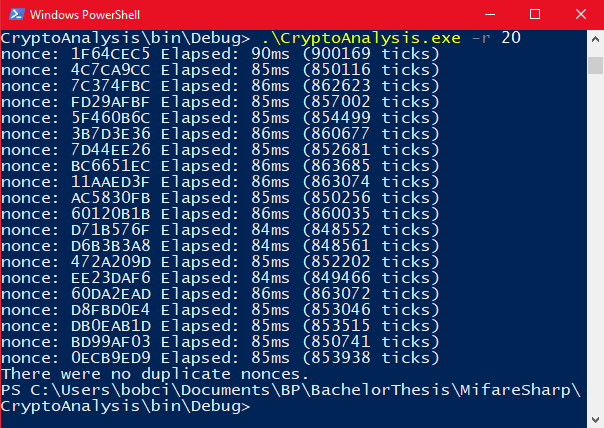
\includegraphics[width=\linewidth]{obrazky-figures/obrazekKryptoanalyza.png}\\[1pt]  
  \caption{Výsledek časové kryptoanalýzy (pro názornost pouze 20 pokusů)}    
  \label{obrazekKryptoanalyza}
\end{figure*}

Program postupně provádí pokusy o autentizace a zaznamenává si výsledné výzvy karty. Po dokončení zadaného množství pokusů jsou v seznamu výzev nalezeny duplikáty. Jak je vidět na obrázku \ref{obrazekKryptoanalyza}, žádné duplikáty nalezeny nebyly. Toto chování se opakovalo i při zvýšení počtu pokusů. Kapitola \ref{predvidatelne_nonce} představuje řešení slabiny karet vydáním novější verze Mifare Classic EV1. Na první pohled by se tak mohlo zdát, že cílová karta je tato novější verze, ale identifikace Chameleonem, příkazem \verb|Identify|, říká, že karta je původní Mifare Classic. Kromě použití příkazu \verb|Identify| si lze také všimnout UID karty. Zatímco délka UID testované karty jsou 4B, nové karty mají UID 7B dlouhé\cite{Mifare_Classic_Official_about}. Z toho vyplývá, že karta samotná není důvod neúspěchu analýzy.\par
Důvodu si můžeme všimnout na obrázku výsledku. Můžeme na něm vidět výsledek dvaceti pokusů o autentizaci. Každý řádek vyjadřuje jeden pokus. Na řádku jsou vždy tři veličiny - přijatá výzva, uplynulý čas daného cyklu v milisekundách a v počtu cyklů procesoru. Předpokladem pro úspěch analýzy je precizní časování v řádu mikrosekund. Jednotlivé pokusy se neliší jen v počtu cyklů procesoru, ale také v milisekundách. Tyto nerovnosti jsou způsobeny možným přepínáním kontextu procesů plánovačem CPU a komunikace sériového portu, který je připojen přes sběrnici USB. Všechna data přenášená tímto způsobem jsou nahrávána do vyrovnávací paměti a jejich doba odeslání se může lišit\cite{RelayUtokBP}.\par
Oba důvody by mohly být vyřešeny použitím specializovaného hardware s možností preciznějšího časování pokusů. Tím může být například už zmíněný Proxmark 3, který obsahuje programovatelná hradlová pole FPGA\cite{Proxmark}. Analýza by tak mohla být prováděna ze zařízení, čímž by se eliminoval přenos přes USB a logika by byla naprogramována přímo v hardware, bez jiných procesů vyžadujících pozornost procesoru. \par
Tato demonstrace se do reálného prostředí příliš nehodí a je vhodná spíše do laboratorních podmínek. Je využitelná při kryptografické analýze karet Mifare Classic a jejich šifry CRYPTO1. 

\section{Emulace karet}
Předmětem další demonstrace je schopnost zařízení Chameleon Mini emulovat karty. Emulací rozumíme schopnost zařízení imitovat kartu při komunikaci s cizím čtecím zařízením. Aby mohla být emulace dostatečně důvěryhodná, musí zařízení pracovat stejně jako původní karta a mít k tomu dostatečné množství dat karty. Chameleon v současné době dokáže emulovat až 5 různých typů karet. Množství potřebných dat závisí na složitosti systému. Některé systémy mohou pracovat přímo s datovými či hodnotovými bloky karty, jiným stačí pouze autentizace karty. Samotným zařízením Chameleon Mini lze získat pouze UID karty. Pro získání celé paměti karty jsou potřeba sofistikovanější zařízení, například ProxMark 3 nebo standardní čtecí zařízení ve spojení s kryptoanalytickými skripty Mifare Classic Universal toolKit (MFCUK) a Mifare Classic Offline Cracker (MFOC)\cite{RelayUtokBP}. Tyto skripty využívají slabin popsaných v kapitole \ref{zranitelnosti}.
Můžeme ale emulovat jen prázdnou kartu s nastaveným UID. Toto řešení nebude fungovat na všechny systémy, pouze na ty, kterým k ověření stačí úspěšná antikolizní fáze s platným UID.\par

\subsection{Nastavení zařízení Chameleon Mini}
Pro emulaci karty je nutné nastavit Chameleon Mini do správné konfigurace. Nejprve zjistíme typ emulované karty příkazem \verb|Identify|.

\begin{lstlisting}[caption=Záznam postupu identifikace karty, label={ChameleonIdentify}]
Config=ISO14443A_READER
100:OK
Identify
101:OK WITH TEXT
Mifare Classic 1k
ATQA:   0400
UID:    9E314C87
SAK:    08
\end{lstlisting}

Správně nastavíme konfiguraci a UID zařízení a je možné přistoupit k demonstraci.

\begin{lstlisting}[caption=Záznam nastavení emulace karty, label={ChameleonSetting}]
Config=MF_CLASSIC_1K
100:OK
Uid=9E314C87
100:OK
\end{lstlisting}

V lednu 2018 byla do firmware Chameleon Mini implementována funkce zjednodušující emulaci karet. Příkaz \verb|Clone| přepne zařízení do konfigurace čtečky, identifikuje přiloženou kartu a správně nakonfiguruje zařízení. Tato funkce lze také navázat na tlačítko (\verb|Rbutton=clone|) a klonovat karty přímo v terénu, bez použití nápadného počítače.

\subsection{Provedení útoku}
\begin{figure*}[ht]\centering
  \centering
  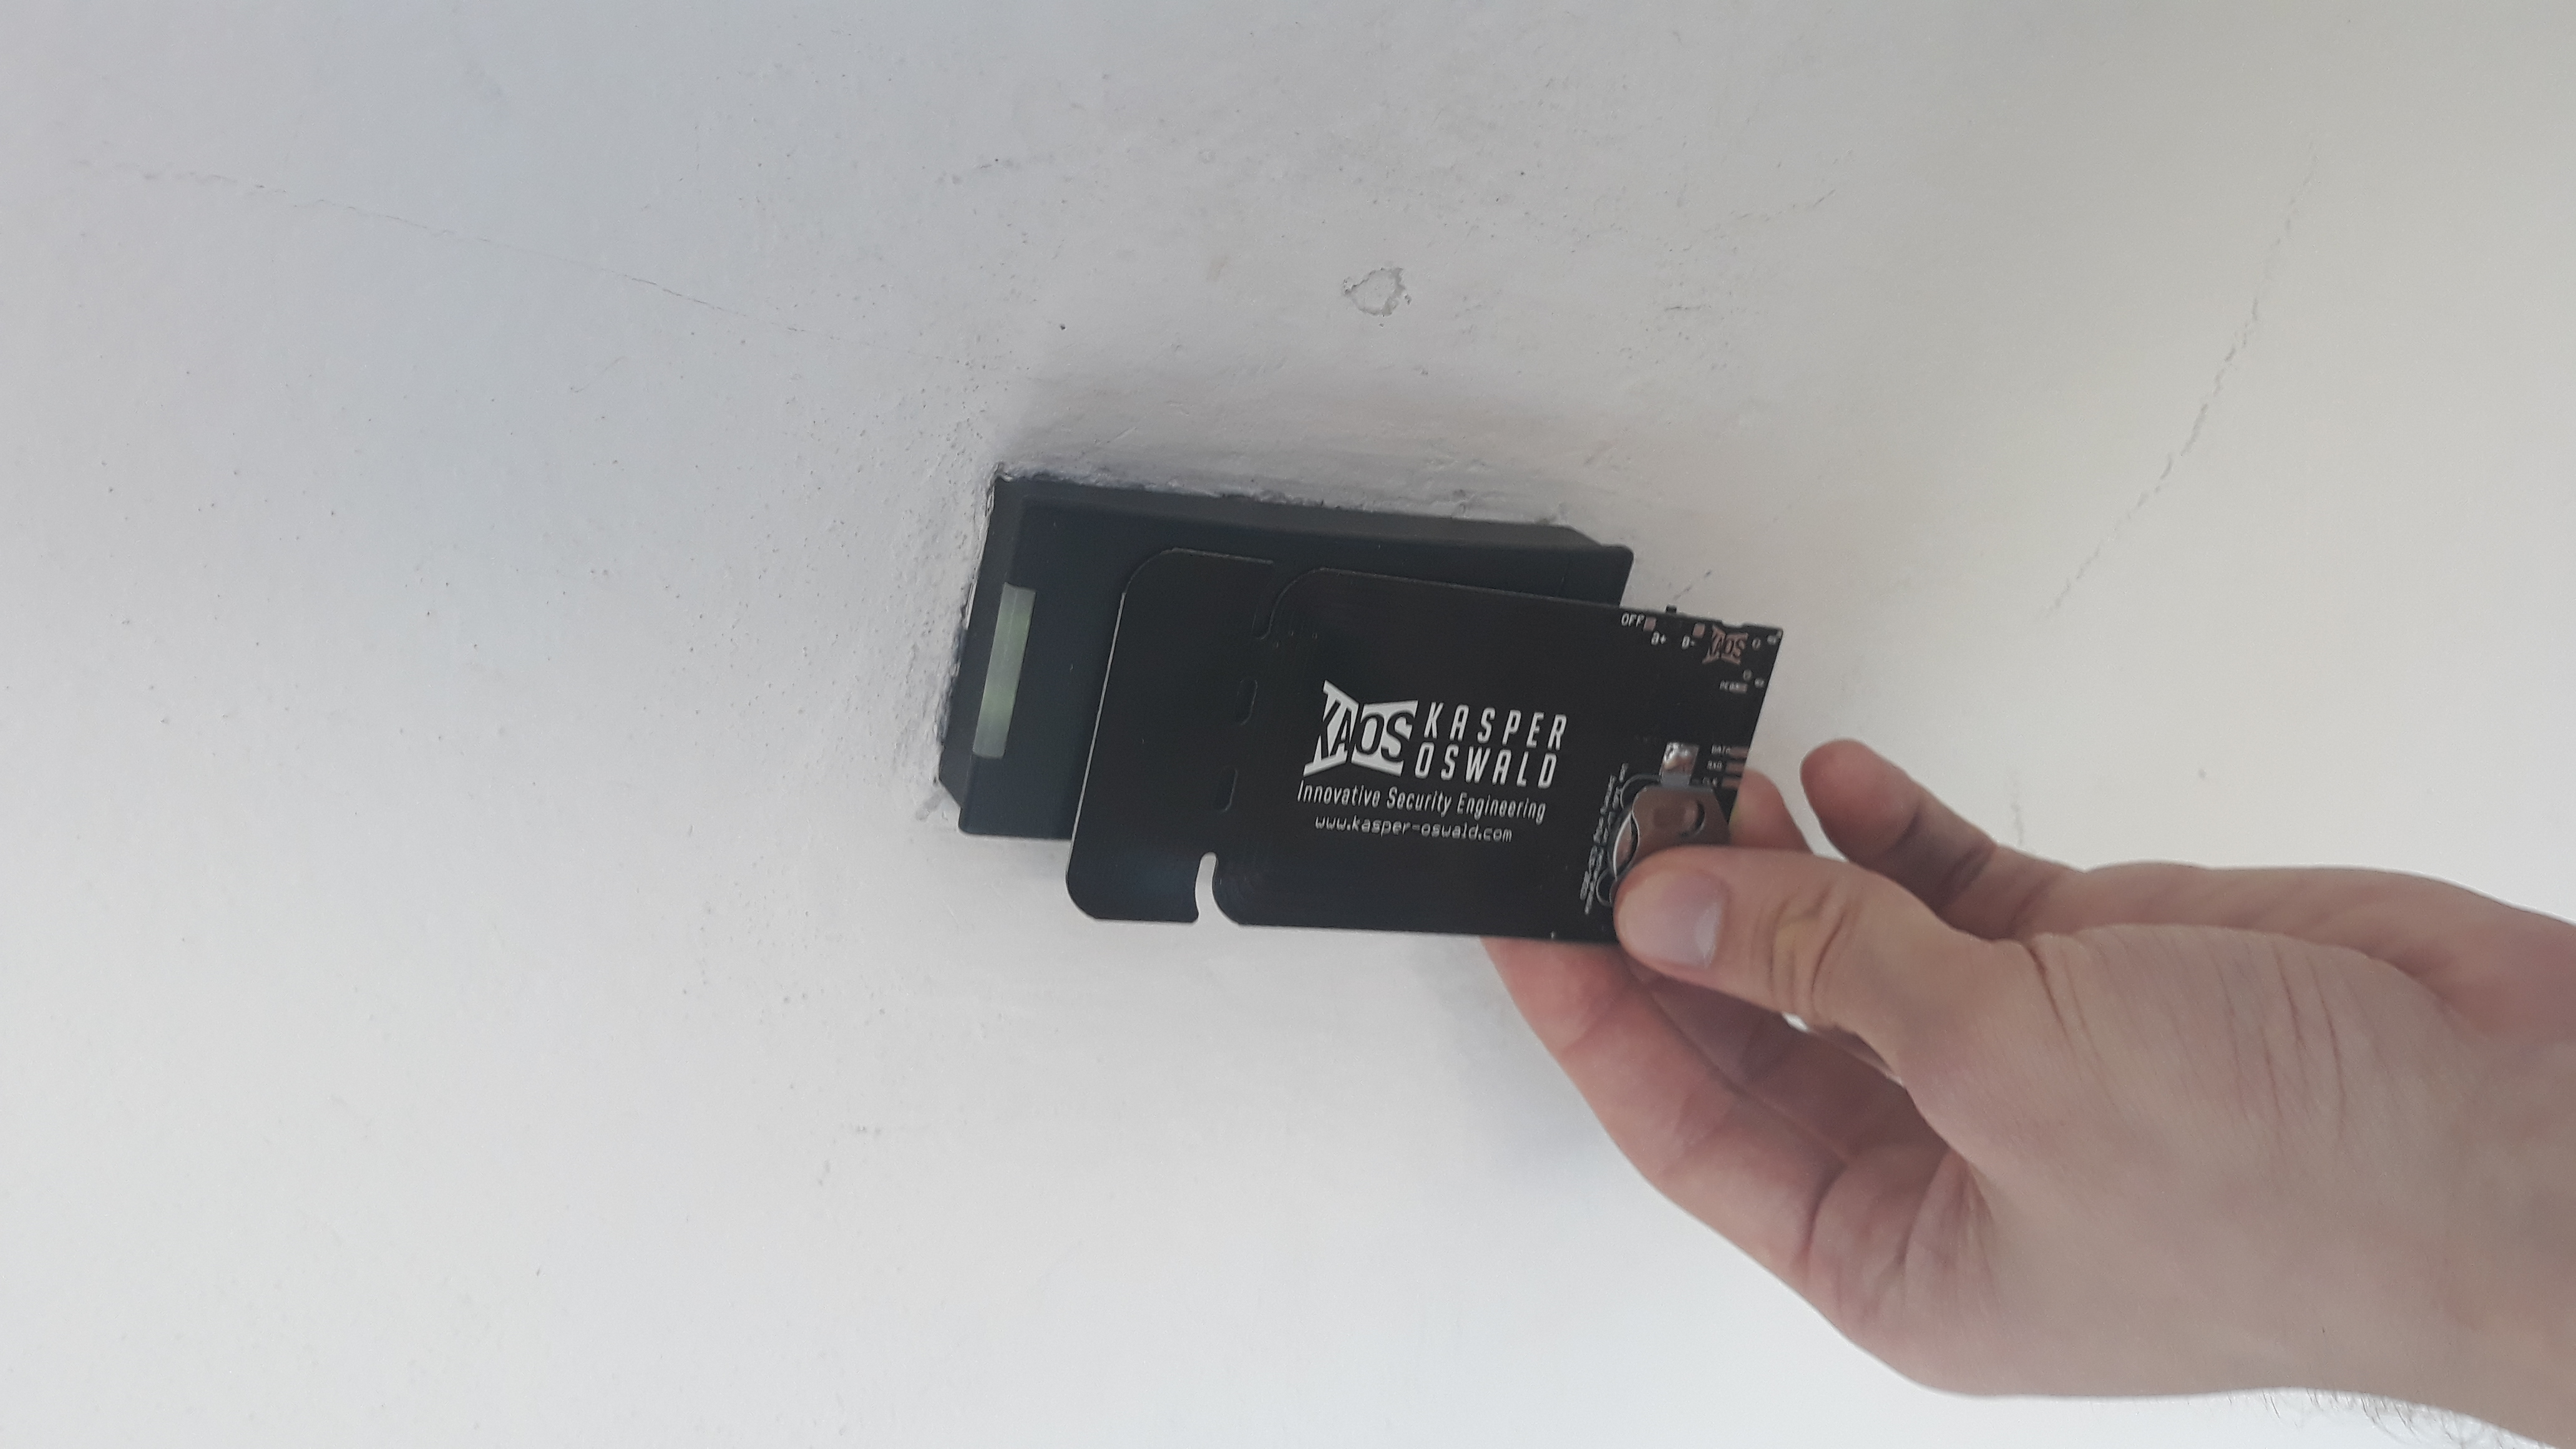
\includegraphics[width=\linewidth, angle=270]{obrazky-figures/obrazekPokusEmulace.jpg}\\[1pt]  
  \caption{Testování emulace karty}    
  \label{obrazekPokusEmulace}
\end{figure*}
Po zapnutí se Chameleon chová stejně jako nakonfigurovaná karta a přiložením ke čtecímu zařízení odpovídá na jeho dotazy. Tento test skončil úspěšně. Po přiložení se světlo na čtecím zařízení rozsvítilo zeleně (patrné i na obrázku \ref{obrazekPokusEmulace}), signalizující úspěšnou identifikaci uživatele. To potvrdilo i následné odemčení vstupních dveří. K identifikaci a vstupu na fakultu tak stačí pouze úspěšná antikolizní fáze. Systém tak získá pouze UID uživatelovy karty a případná další potřebná data získá z vnitřní databáze. To můžeme vidět i na záznamu komunikace čtecího zařízení (viz výpis \ref{emulaceZaznam}). Tento výpis zobrazuje část z logů zařízení Chameleon Mini. Každý záznam (řádek) obsahuje čtyři informace. První dvě se týkají času přijetí, přesněji čas přijetí od startu zařízení a rozdíl časů aktuálního a předchozího přijetí. Druhé dvě se týkají velikosti a obsahu přijatých zpráv. Za povšimnutí stojí, že neproběhne pouze jedna identifikace uživatele. Čtecí zařízení provádí antikolizní algoritmus zhruba každých 100ms. 
\par
\begin{lstlisting}[caption=Část komunikace čtecího zařízení, label={emulaceZaznam}]
04467 ms <  +102 ms>:      (1   bytes) [26                  ]
04468 ms <    +1 ms>:      (2   bytes) [9320                ]
04470 ms <    +2 ms>:      (9   bytes) [93709e314c87644b91  ]
04471 ms <    +1 ms>:      (4   bytes) [500057cd            ]
04573 ms <  +102 ms>:      (1   bytes) [26                  ]
04573 ms <    +0 ms>:      (2   bytes) [9320                ]
04575 ms <    +2 ms>:      (9   bytes) [93709e314c87644b91  ]
04576 ms <    +1 ms>:      (4   bytes) [500057cd            ]
\end{lstlisting}

Po prolomení CRYPTO1 se systémy využívající karty s tímto šifrováním spoléhají pouze na UID, které je uloženo jen pro čtení. Jak je ale vidět z provedeného útoku, není to nejbezpečnější metoda. Chameleon Mini lze za předchozího správného nastavení použít úplně samostatně (bez počítače k ovládání) a provádět tento typ útoku přímo v terénu. Útočník tak pomocí tohoto zařízení může, s trochou nenápadnosti, napadnout jakýkoliv systém využívající podporované karty. Kromě dedikovaných zařízení na emulaci karet, jako je zde použité Chameleon Mini, se dají sehnat čínské kopie karet Mifare Classic s měnitelným UID.  \par
Ke zvýšení zabezpečení systému z pohledu chytrých karet doporučuje i sama firma NXP Semiconductors využít novější typy karet se silnějším šifrováním. Je ale nutné si uvědomit, že bezpečnost se nedá zařídit pouze moderními kartami. Důležitá je celková architektura zabezpečení systému. Není nutné opatřovat si složité zařízení schopné jakéhokoliv útoku, pokud si stačí pro vstup vybrat například jiné dveře, které nevyžadují identifikaci. Dalšími způsoby podobného prolamování bezpečnosti se zabývá sociální inženýrství.\par

\section{Relay útok}

Poslední demonstrací je takzvaný relay útok. Jedná se o {man-in-the-middle} útok. Většina typů autentizací je založena na ujištění, že oba účastníci znají sdílený tajný klíč. Po autentizaci je veškerá komunikace šifrována tímto tajným klíčem a pokud by útočník odposlechl takovou komunikaci, bez znalosti klíče jsou přenášená data stále zabezpečena. Bezkontaktní karty pracují na dálku (do 10cm) a jsou aktivovány vstupem do blízkosti čtecího zařízení. Útočník tak může bez vědomí vlastníka navázat spojení s kartou pomocí vlastního čtecího zařízení a přeposílat komunikaci druhému útočníkovi u vzdáleného čtecího zařízení. Přijatou komunikaci čtecímu zařízení druhý útočník předá, to usoudí, že karta, a tedy i její legitimní uživatel, jsou v blízkosti a vpustí útočníka. Ve skutečnosti může být karta vzdálená několik kilometrů. Data mezi kartou a čtecím zařízením lze posílat jakýmkoliv dostatečně rychlým, přenosovým médiem ({Wi-Fi}, 4G mobilní síť apod.). Přenášené zprávy sice nebudou pro útočníka čitelné, dokud je ale dokáže nezměněné přeposílat včas, tak mu to nevadí. Výhodou takového útoku je nezávislost na šifrovacím algoritmu systému.\par

Pro uskutečnění relay útoku jsou nutná minimálně dvě zařízení, v tomto případe Chameleon Mini, propojená komunikační vrstvou. První zařízení se tváří jako legitimní čtecí zařízení a komunikuje s kartou oběti. Toto zařízení je označováno jako Mole. Druhé zařízení komunikuje s legitimním čtecím zařízením a tváří se jako karta oběti. V literatuře bývá označováno jako Proxy.\cite{PracticalRelayAttack} \par


\begin{figure*}[ht]\centering
  \centering
  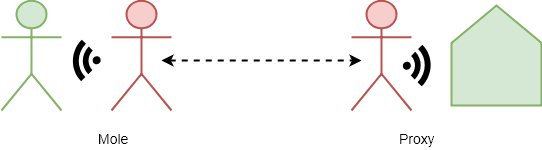
\includegraphics[width=\linewidth]{obrazky-figures/relayAttack.png}\\[1pt]  
  \caption{Schéma relay útoku}    
  \label{obrazekRelayAttack}
\end{figure*}
Program nejprve provede antikolizní fázi mezi Mole a kartou a poté, s daty přijatými od karty, provede antikolizní fázi mezi Proxy a cílovým čtecím zařízením. Z předchozí demonstrace víme, že toto bude stačit k úspěšnému útoku na bezpečnostní systém dveří. Relay útok je ale univerzální a po antikolizní fázi pokračuje v přenášení komunikace. 

\subsection{Implementace}

Implementace útoku je rozdělena na dvě hlavní části. První část je zjednodušený celý útok tak, že zařízení Mole i Proxy jsou připojeny k jednomu programu a data se vyměňují takřka okamžitě v jednom procesu. Jedná se o ověření konceptu útoku. Druhá část už zahrnuje komunikační vrstvu, a je tak možné komunikovat s jiným počítačem. Obě části jsou obsaženy v programu \emph{MifareProxy.exe} a je mezi nimi možné přepínat pomocí argumentů. Implementace opět využívá knihovny \verb|MifareModules|. Aby mohly obě dvě zařízení využívat příkaz \verb|Send|, jsou přepnuty do konfigurace čtecího zařízení.
\par

\subsection*{Jednoduchý relay útok}
Jednoduchý relay útok je standardní chování programu a je spíše demonstračního charakteru. Nejprve jsou inicializovány pomocné moduly pro komunikaci s oběma zařízeními Chameleon Mini. Program předpokládá, že jsou na portech ''COM3'' pro Proxy a ''COM4'' pro Mole. Případně je lze změnit argumenty ''--pcom'', respektive ''--mcom''. Následuje relay útok. Nejprve je provedena antikolizní fáze s kartou oběti. S odpověďmi je provedena antikolizní fáze také s cílovým čtecím zařízením. Poslední zpráva obsahující výzvu k autentizaci je odeslána kartě a ve smyčce se pak vyměňují data mezi zařízeními Mole a Proxy.

\subsection*{Relay útok přes síť}
Pro relay útok s komunikací přes síť je nutné nastavit program do módu Proxy argumentem ''-p'' a do módu Mole argumentem ''-m''. Jméno sériového portu se nastaví stejným způsobem jako u jednoduché verze. Komunikace probíhá přes TCP soket, kdy Proxy je klient a připojuje se k serveru Mole. Adresa~IP a port serveru je potřeba nastavit v obou instancích programu argumenty ''--mip'' a ''--mport''. \par
Nejprve se opět inicializují obě zařízení Chameleon Mini. Po inicializaci vytvoří Mole server a počká na připojení Proxy. Připojením je vše připraveno k útoku. Jeho logika je prakticky stejná jako u jednoduchého útoku, s tím rozdílem, že data jsou posílána sítí a ne pouze sdílenou pamětí. Při komunikaci po síti se může vyskytnout problém s dlouhou dobou doručení, neboli latencí. Tento problém je nejmarkantnější u antikolizní fáze, neboť při ní mají čtečky striktní časování. Nejprve se tedy provede antikolizní fáze s kartou, která nemá striktní časování, a přijatá data karty se odešlou Proxy. Proxy tak má k dispozici veškerá data nutná k této fázi a v jejím průběhu na straně Proxy nemusí probíhat časově náročná síťová komunikace s Mole. 

\subsection{Provedení}

\begin{figure*}[ht]\centering
  \centering
  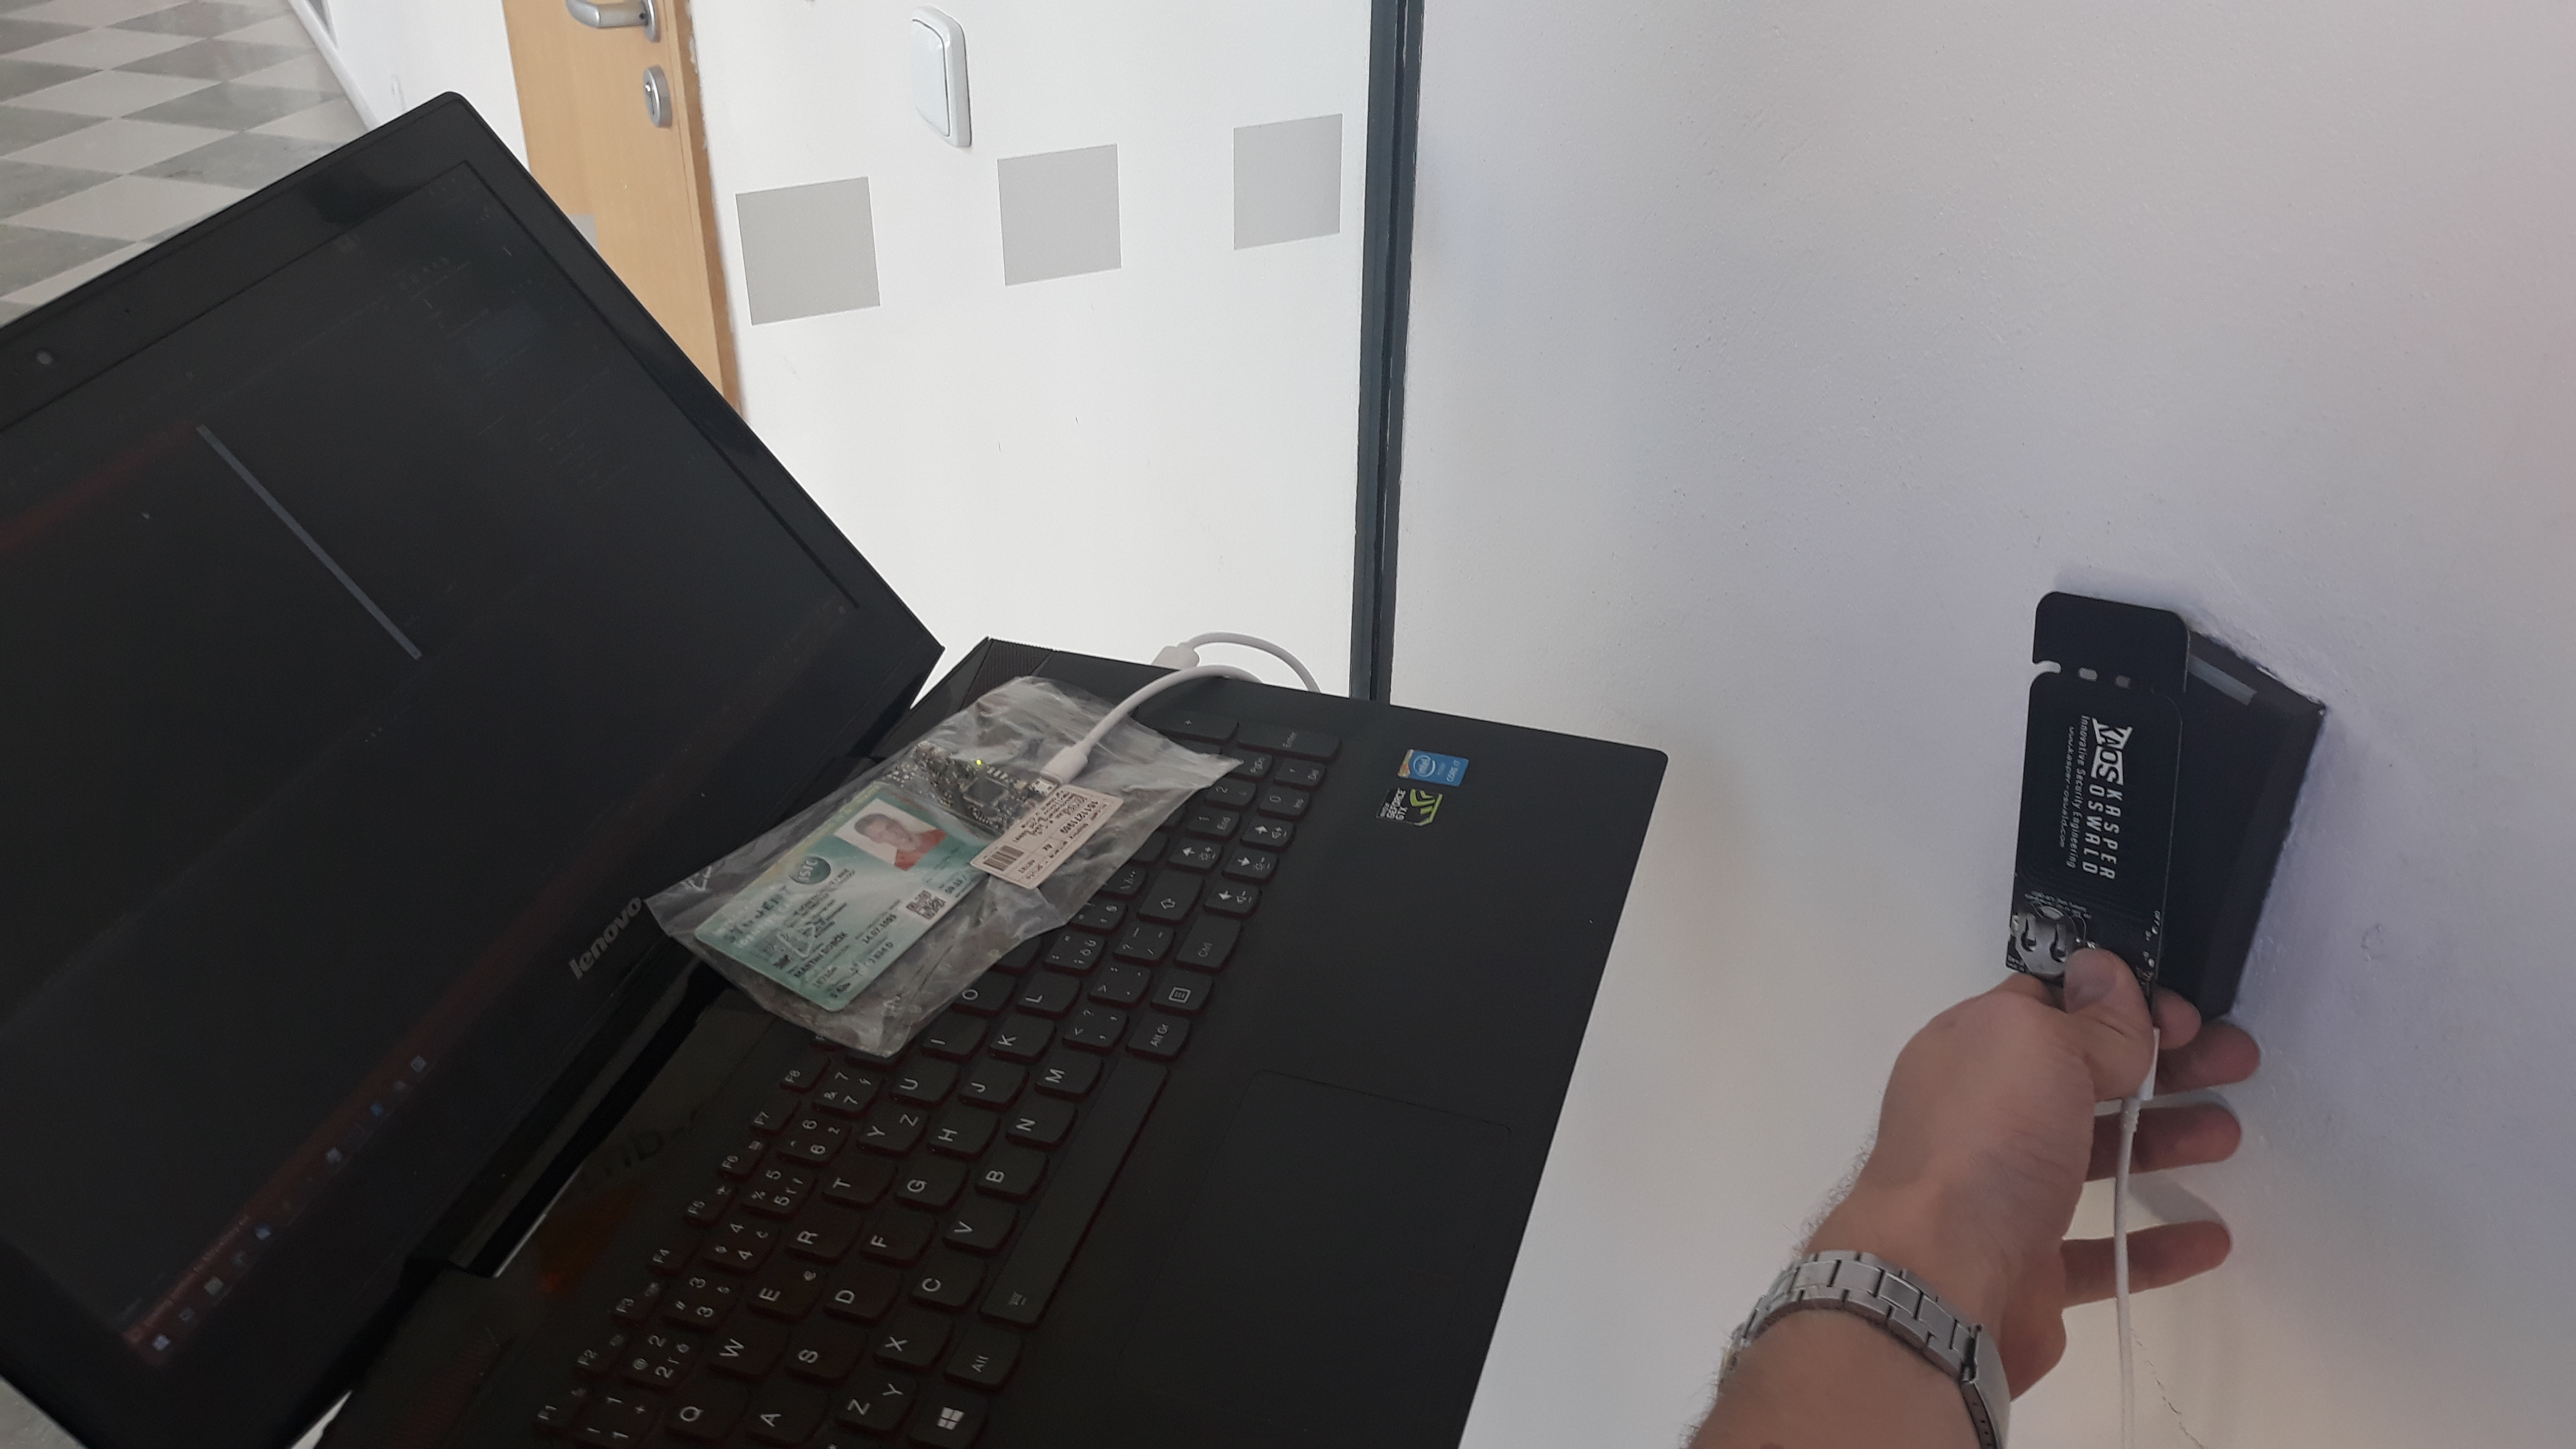
\includegraphics[width=\linewidth]{obrazky-figures/obrazekPokusRelay.jpg}\\[1pt]  
  \caption{Testování relay útoku}    
  \label{obrazekPokusRelay}
\end{figure*}

\begin{lstlisting}[caption=Výstup programu MifareProxy.exe při demonstraci, label={relayZaznam}]
** Chameleon Connected  via COM3 **
** Chameleon Connected  via COM4 **
>ReqA
Mole - SEND 0007 26
<NO DATA
>ReqA
Mole - SEND 0007 26
<0400
>Select
Mole - SEND 0010 9320
<9E314C8764
>Select(9E314C8764)
Mole - SEND 0048 93709E314C87644B91
<Ack (08B6DD)
*** anticollision on mole passed ***
Proxy - SEND 0010 0400
Proxy - < Received NO DATA
Proxy - SEND 0028 9E314C8764
Proxy - < Received NO DATA
Proxy - SEND 0018 08B6DD
Proxy - < Received NO DATA
\end{lstlisting}
Z výstupu programu při provádění relay útoku vidíme, že první část - antikolizní fáze mezi Mole a kartou, skončila úspěšně. Druhá část už úspěšná nebyla a celý útok tak skončil neúspěchem. Proxy sice odeslala data karty, ale čtecí zařízení neodeslalo žádnou odpověď. Z neodemčených dveří lze usoudit, že čtecím zařízením nebyla přijata data. Chameleon Mini v roli Proxy v útoku předstírá, že je karta. Přepnutím zařízení do konfigurace karty se však deaktivuje příkaz \verb|Send| a nelze tak odesílat žádná data\cite{ChameleonDocs}. \par
\begin{lstlisting}[caption=Příkaz Send po přepnutí do konfigurace karty nefunguje, label={NefungujiciSend}]
Config?
101:OK WITH TEXT
ISO14443A_READER
Send 52
101:OK WITH TEXT
0400
0010
PARITY OK
Config=MF_CLASSIC_1K
100:OK
Send 52
201:INVALID COMMAND USAGE
\end{lstlisting}

\subsection{Vyhodnocení}
Neúspěšně odeslaná data lze připsat zařízení Chameleon Mini, které v konfiguraci čtecího zařízení vytváří vlastní elektromagnetické pole\cite{ChameleonDocs}, jímž komunikuje. Cílové čtecí zařízení však očekává modulaci jeho nosné vlny (viz část \ref{pasivniTagy}), což se neděje. Z předchozí demonstrace víme, že Chameleon Mini dokáže se čtecím zařízením komunikovat, avšak pouze v konfiguraci emulace karty. Tato konfigurace pouze pasivně emuluje kartu a nelze se aktivně zapojovat do komunikace pomocí komunikačního portu\cite{ChameleonDocs}. Relay útok za pomoci zařízení Chameleon Mini je tak možný pouze částečně, v roli Mole. Pro roli Proxy je nutné využít jiného zařízení, například již zmiňovaného Proxmark3 nebo standardní čtecí zařízení umožňující emulaci karet\cite{RelayUtokBP}. Druhou možností je implementace odesílání dat v konfiguraci emulace karet do open source firmware Chameleon Mini. Zde by se ovšem mohl vyskytnout problém z první demonstrace (viz část\ref{casovaKryptoanalyza}), kdy USB sběrnice zvyšuje latenci.\par
Vzhledem k tomu, že relay útok je nezávislý na šifrování karty, je zabezpečení proti němu omezené. Nejzákladnější ochranou je uzavřít kartu při přenosu Faradayovy klece, které zabrání vstupu elektromagnetického pole ke kartě. Při používání je však nutno kartu z klece vyjmout, čímž vzniká krátké okno k provedení útoku. Další metodou může být zadáváním PIN kódu při jakékoliv manipulaci s kartou. Dále je možné detekovat vzdálenost karty a relay útok pomocí takzvaných {distance-bounding} protokolů, které ale zatím nevyužívá žádný standard.\par
Tento útok je možné v praxi využít. Jsou potřeba dva útočníci. První, v roli Mole, se musí přiblížit ke kartě oběti na dostatečně dlouhou dobu potřebnou k přenesení informací. To je možné například v plné hromadné dopravě nebo při čekání v řadě. Samotná doba přenesení jedné autentizace je krátká, je ovšem nutné vzít v úvahu opakovaní útoku vícekrát z důvodu možného narušení přenosu. Útočník v roli Proxy musí nenápadně přiložit zařízením do blízkosti čtečky. Na takovém místě většinou bývá jiné zabezpečení v podobě kamer či bezpečnostní služby a neznámý předmět by vyvolal rozruch. Je ale možné zařízení zavřít do peněženky či brašny kde bude nenápadné, stejné jako normální karty.\cite{PracticalRelayAttack}


\chapter{Závěr}
\label{zaver}
Cílem této práce bylo seznámit se s kartami Mifare Classic se zaměřením na jejich zranitelnosti a demonstrovat vybrané zneužitelnosti za pomoci zařízení Chameleon Mini. \par
Studiu technologie RFID a kartám Mifare Classic byly věnovány první dvě kapitoly. Samotné zranitelnosti těchto karet byly rozebrány v kapitole následující. Zadáním bylo určeno, že demonstrace vybraných zranitelností má být provedeno pomocí zařízení Chameleon Mini, bylo tedy nastudováno také jeho využití a možnosti.
Na základě informací o komunikačním protokolu a šifrovacím algoritmu těchto karet byly navrženy a provedeny tři demonstrace, z nichž dvě vyžadovaly také implementační část. Ta byla provedena v jazyce C\#.Net a byla vytvořena pomocná knihovna pro usnadnění práce se zařízením Chameleon Mini.\par
Časová kryptoanalýza se zabývala nedostatečnou náhodností generátoru náhodných čísel, který používá šifrovací algoritmus karty. Následoval útok nevyžadující implementaci, při kterém zařízení Chameleon Mini naklonuje a emuluje cizí kartu. Jako poslední byl proveden takzvaný relay útok, který přenáší komunikaci mezi kartou oběti a legitimním čtecím zařízením. Z těchto demonstrací lze považovat pouze útok s emulovanou kartou jako zcela úspěšný. Zbylé dvě demonstrace se nepodařily kvůli nedostatečným schopnostem zařízení Chameleon Mini. Všechny demonstrace byly provedeny v reálném prostředí na dveřích osazených čtecím zařízením HID RP10.\par

Pokračovat v této práci lze více směry. Jelikož zařízení Chameleon Mini nemělo dostatečné schopnosti pro dva ze tří útoků, nabízí se možnost provést stejné útoky za použití jiných zařízení, případně rozšířit firmware Chameleon Mini o potřebnou funkcionalitu, která prováděné útoky umožní. Dále je možné provést analýzu a útoky na jiné typy karet, nebo rozšířit paletu útoků o další.\par












